\section{Numerical Results}
\label{sec:results}

To test and verify the implementation of the quadtree-adaptive HPS method, we solve two Poisson equations and one Helmholtz equation. For each, we present error, timing, and memory usage results and discuss the performance of our implemented method.

For all of our examples, we discretize the Laplace operator at the patch level using a second-order, 5-point stencil on a finite volume (cell-centered) mesh. The code, along with numerical experiments below, is stored in the GitHub repository EllipticForest \citep{chipman2023elliptic}. EllipticForest is written primarily in C++, with wrappers to FORTRAN routines to call FISHPACK and LAPACK (\citep{anderson1999lapack}) for any dense linear algebra operations. The mesh and solution are output into an unstructured VTK mesh file \citep{vtkBook} and are visualized with the VisIt software \citep{HPV:VisIt}. All tests were run on a 2021 MacBook Pro with an M1 Pro CPU and 32 GB of RAM.

\subsection{Poisson Equation 1}
\label{sub:example_one}

We solve the following boundary value problem:
\begin{align}
    \nabla^2 u(x,y) = -(\sin(x) + \sin(y))
\end{align}
on the square domain $\Omega = [-10, 10] \times [-10, 10]$, subject to Dirichlet boundary conditions $u(x,y) = g(x,y)$ on the boundary which is computed according to the exact solution
\begin{align}
    u_{exact}(x,y) &= \sin(x) + \sin(y).
\end{align}

For the refinement criteria, we refine according to the right-hand side function $f(x,y)$, which corresponds to the curvature of the solution. We set a refinement threshold of $1.2$ and refine a patch when $f(x,y) > 1.2$ for any $x,y$ in a patch. This results in a mesh and solution that can be found in \reffig{fig:poisson_plot}.

\begin{figure}
    \centering
    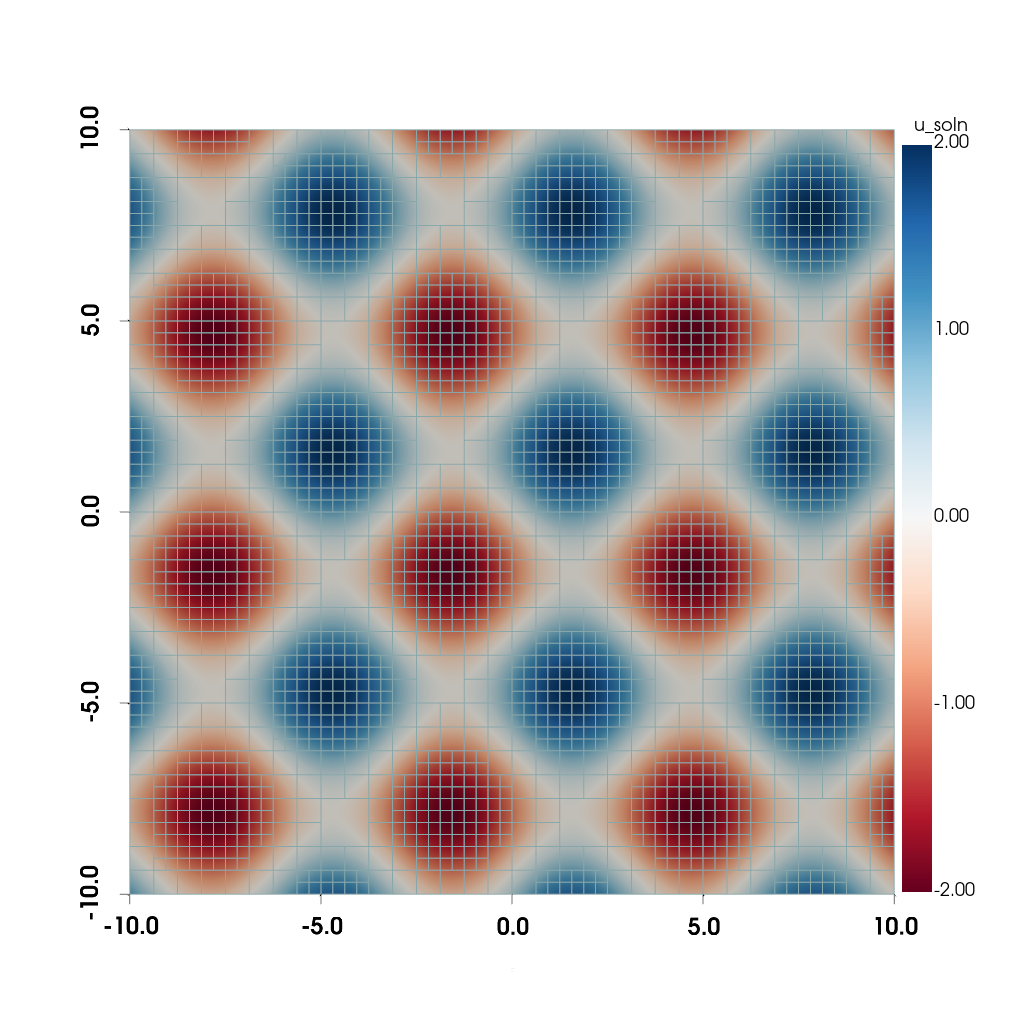
\includegraphics[width=0.75\textwidth, trim={0 100 0 0}]{figures/plot_poisson.png}
    \caption{The computed solution and mesh for the Poisson problem \refsec{sub:example_one}.  Patch size for this plot is $16 \times 16$ and mesh is refined to level 7.  Refinement criteria is based on the magnitude of the right hand side function $f(x,y)$.}
    \label{fig:poisson_plot}
\end{figure}

{\bf Results and Discussion}
Tables \ref{tab:poisson_error} and \ref{tab:poisson_timing} show the error, timing, and memory results for the current implementation on this Poisson equation. \reftab{tab:poisson_error} shows results for both a uniformly refined mesh (a mesh without any coarse-fine interfaces or local adaptivity) and results for the adaptive mesh case. For the uniform case, we get the expected second order convergence in both the $L_{\infty}$ and $L_1$ norms. The adaptive case mostly shows second order convergence, except for a few cases where the refinement between successive levels results in a smaller jump in error than second order provides. \reftab{tab:poisson_timing} shows timing and memory results for the same case. Here, the difference between the uniform and adaptive case is highlighted. The adaptive case gives a $4.5$ times speed up for the build stage, and nearly a $20$ times speed up for the solve stage. Memory used to store the quadtree and operators is also significantly reduced with the adaptive case.

% \begin{table}
%     \caption{TODO}
%     \begin{center}
%         \sisetup{
%             detect-weight=true,
%             detect-inline-weight=math,
%             table-alignment-mode=format
%         }
%         \begin{tabular}{
%             S   % Max levels
%             S   % Effective resolution
%             S   % DOFs
%             S[scientific-notation=true, round-mode=places, round-precision=2]   % L-inf error
%             S[round-mode=places, round-precision=2]   % L-inf order
%             S[scientific-notation=true, round-mode=places, round-precision=2]   % L-1 error
%             S[round-mode=places, round-precision=2]   % L-1 order
%             S[round-mode=places, round-precision=3]   % Build time
%             S[round-mode=places, round-precision=3]   % Solve time
%             S[round-mode=places, round-precision=1]   % Memory size
%         }
% \hline
% {$L$} & {$R_{eff}$} & {DOFs} & {$L_{\infty}$ Error} & {$L_{\infty}$ Order} & {$L_1$ Error} & {$L_1$ Order} & {$T_{B}$ (sec)} & {$T_{S}$ (sec)} & {$B$ (MB)} \\
% \hline
% \num{1} & \num{32} & \num{1024} & \num{0.0727000000000000} & {--} & \num{0.0233000000000000} & {--} & \num{0.0017400000000000} & \num{0.0027700000000000} & \num{0.4280000000000000} \\
% \num{2} & \num{64} & \num{4096} & \num{0.0178000000000000} & \num{2.0300781229532000} & \num{0.0057600000000000} & \num{2.0161892380993300} & \num{0.0120000000000000} & \num{0.0146000000000000} & \num{2.8400000000000000} \\
% \num{3} & \num{128} & \num{16384} & \num{0.0044600000000000} & \num{1.9967616259334600} & \num{0.0014400000000000} & \num{2.0000000000000000} & \num{0.0684000000000000} & \num{0.0448000000000000} & \num{15.9000000000000000} \\
% \num{4} & \num{256} & \num{65536} & \num{0.0011100000000000} & \num{2.0064840335702000} & \num{0.0003590000000000} & \num{2.0040130625066200} & \num{1.4400000000000000} & \num{0.1910000000000000} & \num{81.5000000000000000} \\
% \num{5} & \num{512} & \num{262144} & \num{0.0002790000000000} & \num{1.9922226494082800} & \num{0.0000897000000000} & \num{2.0008039537911500} & \num{7.2000000000000000} & \num{0.8940000000000000} & \num{398.0000000000000000} \\
% \num{6} & \num{1024} & \num{1048576} & \num{0.0000696000000000} & \num{2.0031059108678200} & \num{0.0000224000000000} & \num{2.0016092528616600} & \num{34.1000000000000000} & \num{3.8600000000000000} & \num{1880.0000000000000000} \\
% \num{7} & \num{2048} & \num{4194304} & \num{0.0000174000000000} & \num{2.0000000000000000} & \num{0.0000056100000000} & \num{1.9974260563361700} & \num{160.0000000000000000} & \num{19.0000000000000000} & \num{8680.0000000000000000} \\
% \hline
%         \end{tabular}
%     \end{center}
% \end{table}

\begin{table}
    \caption{Convergence analysis for Poisson's equation. The upper part shows convergence for a uniformly refined mesh, while the lower part shows convergence for an adaptively refined mesh. $M$ is the size of the grid on each leaf patch, $L_{\text{max}}$ is the maximum level of refinement, $R_{\text{eff}}$ is the effective resolution for a uniformly refined mesh, DOFs is the total degrees of freedom (i.e., total mesh points), $L_{\infty}$ error is the infinity norm error, $L_{\infty}$ order is the infinity norm convergence order, $L_1$ error is the $1^{\text{st}}$ norm error, and $L_1$ order is the $1^{\text{st}}$ norm convergence order.}
    \centering
    \sisetup{
        table-alignment-mode=format
    }
    \begin{tabular}{
        |
        S   % Patch size
        S[table-column-width=0.8cm]   % Max level
        S[table-text-alignment=right, table-column-width=0.7cm]   % Effective resolution
        S[table-text-alignment=right, table-column-width=1.4cm]   % DOFs
        S[scientific-notation=true, round-mode=places, round-precision=2, table-column-width=1.65cm]   % L-inf error
        S[scientific-notation=false, exponent-mode=fixed, round-mode=places, round-precision=2, table-column-width=1.5cm]   % L-inf order
        S[scientific-notation=true, round-mode=places, round-precision=2]   % L-1 error
        S[scientific-notation=false, exponent-mode=fixed, round-mode=places, round-precision=2]   % L-1 order
        |
    }
\hline
{M} & {$L_{\text{max}}$} & {$R_{\text{eff}}$} & {DOFs} & {$L_{\infty}$ Error} & {$L_{\infty}$ Order} & {$L_1$ Error} & {$L_1$ Order} \\
\hline
% \num{16} & \num{1} & \num{32} & \num{1024} & \num{7.2721827038740E-02} & {--} & \num{2.3319531214882E-02} & {--} \\
% \num{16} & \num{2} & \num{64} & \num{4096} & \num{1.7803276283615E-02} & \num{2.0302456853013E+00} & \num{5.7570511934287E-03} & \num{2.0181368404886E+00} \\
% \num{16} & \num{3} & \num{128} & \num{16384} & \num{4.4594278588197E-03} & \num{1.9972122300096E+00} & \num{1.4365857848192E-03} & \num{2.0026858961169E+00} \\
\num{16} & \num{4} & \num{256} & \num{65536} & \num{1.1146466297640E-03} & \num{2.0002722123237E+00} & \num{3.5892082197986E-04} & \num{2.0009066196875E+00} \\
\num{16} & \num{5} & \num{512} & \num{262144} & \num{2.7855514231123E-04} & \num{2.0005515585727E+00} & \num{8.9717104596707E-05} & \num{2.0002106534890E+00} \\
\num{16} & \num{6} & \num{1024} & \num{1048576} & \num{6.9642847198903E-05} & \num{1.9999158585307E+00} & \num{2.2428541266291E-05} & \num{2.0000472698832E+00} \\
\num{16} & \num{7} & \num{2048} & \num{4194304} & \num{1.7410906046011E-05} & \num{1.9999839043577E+00} & \num{5.6070914295010E-06} & \num{2.0000112920243E+00} \\
% \num{32} & \num{1} & \num{64} & \num{4096} & \num{1.7803276283615E-02} & {--} & \num{5.7570511934284E-03} & {--} \\
% \num{32} & \num{2} & \num{128} & \num{16384} & \num{4.4594278588175E-03} & \num{1.9972122300103E+00} & \num{1.4365857848190E-03} & \num{2.0026858961170E+00} \\
% \num{32} & \num{3} & \num{256} & \num{65536} & \num{1.1146466297716E-03} & \num{2.0002722123132E+00} & \num{3.5892082198209E-04} & \num{2.0009066196784E+00} \\
\num{32} & \num{4} & \num{512} & \num{262144} & \num{2.7855514234232E-04} & \num{2.0005515584215E+00} & \num{8.9717104608167E-05} & \num{2.0002106533137E+00} \\
\num{32} & \num{5} & \num{1024} & \num{1048576} & \num{6.9642847325024E-05} & \num{1.9999158560790E+00} & \num{2.2428541313515E-05} & \num{2.0000472670298E+00} \\
\num{32} & \num{6} & \num{2048} & \num{4194304} & \num{1.7410906499649E-05} & \num{1.9999838693813E+00} & \num{5.6070916187308E-06} & \num{2.0000112463735E+00} \\
\hline
% \num{16} & \num{1} & \num{32} & \num{1024} & \num{7.2721827038740E-02} & {--} & \num{2.3319531214882E-02} & {--} \\
% \num{16} & \num{2} & \num{64} & \num{4096} & \num{1.7803276283615E-02} & \num{2.0302456853013E+00} & \num{5.7570511934287E-03} & \num{2.0181368404886E+00} \\
% \num{16} & \num{3} & \num{128} & \num{16384} & \num{4.4594278588197E-03} & \num{1.9972122300096E+00} & \num{1.4365857848192E-03} & \num{2.0026858961169E+00} \\
\num{16} & \num{4} & \num{256} & \num{64000} & \num{2.5910957992683E-03} & \num{7.8329626881446E-01} & \num{4.4586170147130E-04} & \num{1.6879759592817E+00} \\
\num{16} & \num{5} & \num{512} & \num{194560} & \num{6.6263501289099E-04} & \num{1.9672760156010E+00} & \num{1.2477150864153E-04} & \num{1.8373077457909E+00} \\
\num{16} & \num{6} & \num{1024} & \num{569344} & \num{6.8094879278413E-04} & \num{-3.9331876110758E-02} & \num{1.0216613949030E-04} & \num{2.8837140596648E-01} \\
\num{16} & \num{7} & \num{2048} & \num{1984000} & \num{1.7141451745961E-04} & \num{1.9900570123994E+00} & \num{3.7577025980665E-05} & \num{1.4429943340785E+00} \\
% \num{32} & \num{1} & \num{64} & \num{4096} & \num{1.7803276283615E-02} & {--} & \num{5.7570511934284E-03} & {--} \\
% \num{32} & \num{2} & \num{128} & \num{16384} & \num{4.4594278588175E-03} & \num{1.9972122300103E+00} & \num{1.4365857848190E-03} & \num{2.0026858961170E+00} \\
% \num{32} & \num{3} & \num{256} & \num{65536} & \num{1.1146466297716E-03} & \num{2.0002722123132E+00} & \num{3.5892082198209E-04} & \num{2.0009066196784E+00} \\
\num{32} & \num{4} & \num{512} & \num{256000} & \num{6.6189922864102E-04} & \num{7.5190291839197E-01} & \num{1.1198962819648E-04} & \num{1.6803004955197E+00} \\
\num{32} & \num{5} & \num{1024} & \num{784384} & \num{1.6733508690897E-04} & \num{1.9838716073808E+00} & \num{3.1111362539336E-05} & \num{1.8478516397654E+00} \\
\num{32} & \num{6} & \num{2048} & \num{2289664} & \num{1.7139947044398E-04} & \num{-3.4622669955039E-02} & \num{2.5679498208238E-05} & \num{2.7682456821605E-01} \\
\hline
    \end{tabular}
    \label{tab:poisson_error}
\end{table}

\begin{table}
    \caption{Timing and memory results for Poisson's equation. The upper part shows results for the uniformly refined mesh, while the lower part shows results for the adaptively refined mesh. The results here are for a patch size of $16 \times 16$. $L_{\text{max}}$ is the maximum level of refinement, $R_{\text{eff}}$ is the effective resolution, DOFs is the total degrees of freedom, $T_{\text{build}}$ is the time in seconds for the build stage, $T_{\text{upwards}}$ is the time in seconds for the upwards stage, $T_{\text{solve}}$ is the time in seconds for the solve stage, and $S$ is the memory storage in megabytes to store the quadtree and all data matrices stored in each node of the quadtree.}
    \centering
    \sisetup{
        table-alignment-mode=format
    }
    \begin{tabular}{
        |
        S   % Max level
        S[table-text-alignment=right]   % Effective resolution
        S[table-text-alignment=right]   % Total DOFs
        S[table-text-alignment=right, scientific-notation=false, round-mode=places, round-precision=3]   % Build time
        S[table-text-alignment=right, scientific-notation=false, exponent-mode=fixed, round-mode=places, round-precision=3]   % Upwards time
        S[table-text-alignment=right, scientific-notation=false, round-mode=places, round-precision=3]   % Solve time
        S[table-text-alignment=right, scientific-notation=false, round-mode=places, round-precision=1]   % Memory size
        |
    }
\hline
{$L_{\text{max}}$} & {$R_{\text{eff}}$} & {DOFs} & {$T_{\text{build}}$ (sec)} & {$T_{\text{upwards}}$ (sec)} & {$T_{\text{solve}}$ (sec)} & {$S$ (MB)} \\
\hline
% \num{1} & \num{32} & \num{1024} & \num{0.015641083000000} & \num{1.07767500000000E-02} & \num{0.020481166000000} & \num{0.428303718566894} \\
% \num{2} & \num{64} & \num{4096} & \num{0.085338584000000} & \num{2.00472499999999E-02} & \num{0.036223209000000} & \num{2.843113899230950} \\
% \num{3} & \num{128} & \num{16384} & \num{0.393952542000000} & \num{7.48480829999999E-02} & \num{0.059746333000000} & \num{15.882237434387200} \\
\num{4} & \num{256} & \num{65536} & \num{2.031286957999990} & \num{3.66539416999999E-01} & \num{0.211029084000000} & \num{81.548497200012200} \\
\num{5} & \num{512} & \num{262144} & \num{8.525974832999990} & \num{1.77923349999999E+00} & \num{1.073760000000000} & \num{398.233067512512000} \\
\num{6} & \num{1024} & \num{1048576} & \num{39.353658666999900} & \num{9.00205208400000E+00} & \num{4.258692584000000} & \num{1881.010411262510000} \\
\num{7} & \num{2048} & \num{4194304} & \num{172.189544875000000} & \num{4.20349420419999E+01} & \num{20.559359582999900} & \num{8676.197911262510000} \\
\hline
% \num{1} & \num{32} & \num{1024} & \num{0.010200834000000} & \num{2.31674999999999E-03} & \num{0.013967208000000} & \num{0.428303718566894} \\
% \num{2} & \num{64} & \num{4096} & \num{0.077488417000000} & \num{1.34400419999999E-02} & \num{0.016857250000000} & \num{2.843113899230950} \\
% \num{3} & \num{128} & \num{16384} & \num{0.320450292000000} & \num{8.29752079999999E-02} & \num{0.049673459000000} & \num{15.882237434387200} \\
\num{4} & \num{256} & \num{64000} & \num{1.502292208999990} & \num{3.93616458000000E-01} & \num{0.098160250000000} & \num{52.977078437805100} \\
\num{5} & \num{512} & \num{194560} & \num{3.718632625000000} & \num{9.24946582999999E-01} & \num{0.290812499999999} & \num{140.070134162902000} \\
\num{6} & \num{1024} & \num{569344} & \num{10.594630750000000} & \num{2.22070095800000E+00} & \num{0.478022832999999} & \num{368.462132453918000} \\
\num{7} & \num{2048} & \num{1984000} & \num{38.976778125000000} & \num{8.09454862499999E+00} & \num{1.838669208000000} & \num{1443.861859321590000} \\
\hline
    \end{tabular}
    \label{tab:poisson_timing}
\end{table}

\subsection{Poisson Equation 2 (Polar-Star Problem)}

As another test for Poisson's equation, we solve a ``polar star'' Poisson problem. The problem is created via a method of manufactured solutions and is engineered to have highly local curvature from the load function. The resulting solution is a collection of polar stars with user specified number of points and radii of curvature. This problem highlights the use of an adaptive mesh to solve the elliptic equation. The exact solution we attempt to reconstruct is the following:
\begin{align}
    u(x,y) = \frac{1}{2} \sum_{i=1}^{N} 1 - \tanh \left(\frac{r(x,y)-r_{0,i} \left(r_{1,i} \cos \left(n \theta(x,y)\right)+1\right)}{\epsilon }\right)
\end{align}
Computing the Laplacian analytically yields the right-hand side to Poisson's equation. Thus, the polar star Poisson problem is defined as follows:
\begin{align}
    \nabla^2 u(x,y) = \sum_{i=1}^N -\frac{s_{1,i}(x,y) + s_{2,i}(x, y)}{r(x,y)^2} - s_{3,i}(x,y) + s_{4,i}(x,y)
\end{align}
with
\begin{align*}
    s_{1,i}(x,y) &= \frac{p(x,y)^2 \tanh \left(\phi(x,y)\right) \text{sech}^2\left(\phi(x,y)\right)}{\epsilon ^2} \\
    s_{2,i}(x,y) &= -\frac{n^2 r_{0,i} r_{1,i} \cos (n \theta(x,y)) \text{sech}^2\left(\phi(x,y)\right)}{2 \epsilon } \\
    s_{3,i}(x,y) &= \frac{\tanh \left(\phi(x,y)\right) \text{sech}^2\left(\phi(x,y)\right)}{\epsilon ^2} \\
    s_{4,i}(x,y) &= \frac{\text{sech}^2\left(\phi(x,y)\right)}{2 r(x,y) \epsilon } \\
    p(x,y) &= n r_{0,i} r_{1,i} \sin (n \theta(x,y)) \\
    \phi(x,y) &= \frac{r(x,y)-r_{0,i} (r_{1,i} \cos (n \theta(x,y))+1)}{\epsilon}
\end{align*}
and where $i=1, ..., N_{polar}$ and $N_{polar}$ is the number of polar stars. Each polar star has a center $(x_0, y_0)$, inner and outer radii $r_0, r_1$, and the number of arms per polar star $n$. The radius and angle have the standard polar transforms:
\begin{align}
    r(x,y) &= \sqrt{(x - x_0)^2 + (y - y_0)^2} \\
    \theta(x,y) &= \tan^{-1}\Big(\frac{y - y_0}{x - x_0}\Big)
\end{align}
\reftab{table:polar_star_parameters} has the parameters used in this case study. \reffig{fig:polar_star_plot} shows the resulting mesh and solution. \reftab{tab:polar_star_results} shows the error, timing, and memory results for the polar star Poisson problem.
\begin{table}[ht]
    \begin{center}
        \caption{Polar Star Poisson Problem Parameters}
        \begin{tabular}{|c|c|c|c|c|c|}
            \hline
            $i$ & $x_0$ & $y_0$ & $r_0$ & $r_1$ & $n$ \\
            \hline
            $1$ & $-0.5$ & $-0.5$ & $0.2$ & $0.3$ & $3$ \\
            $2$ & $0.5$ & $-0.5$ & $0.3$ & $0.4$ & $4$ \\
            $3$ & $0$ & $0.5$ & $0.4$ & $0.5$ & $5$ \\
            \hline
        \end{tabular}
        \label{table:polar_star_parameters}
    \end{center}
\end{table}

\begin{figure}
    \centering
    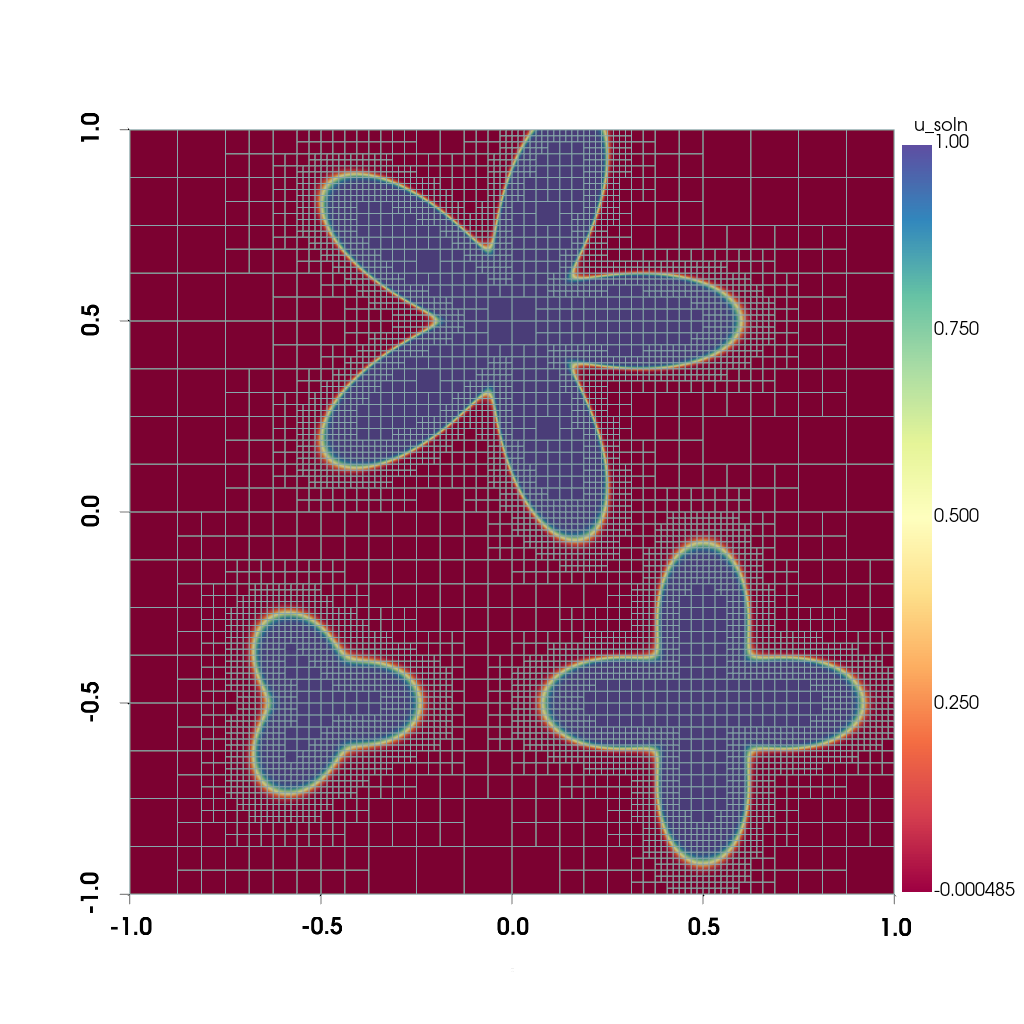
\includegraphics[width=0.75\textwidth, trim={0 100 0 0}]{figures/plot_polar_star.png}
    \caption{The computed solution and mesh for the Polar Star Poisson problem. Each patch has a $16 \times 16$ cell-centered grid. The mesh is refined according to the right-hand side and is refined with 8 levels of refinement.}
    \label{fig:polar_star_plot}
\end{figure}

\begin{table}
    \caption{Convergence analysis for the Polar Star Poisson problem. The upper part shows convergence for a uniformly refined mesh, while the lower part shows convergence for an adaptively refined mesh. $M$ is the size of the grid on each leaf patch, $L_{\text{max}}$ is the maximum level of refinement, $R_{\text{eff}}$ is the effective resolution for a uniformly refined mesh, DOFs is the total degrees of freedom (i.e., total mesh points), $L_{\infty}$ error is the infinity norm error, $L_{\infty}$ order is the infinity norm convergence order, $L_1$ error is the $1^{\text{st}}$ norm error, and $L_1$ order is the $1^{\text{st}}$ norm convergence order.}
    \centering
    \sisetup{
        table-alignment-mode=format
    }
    \begin{tabular}{
        |
        S   % Patch size
        S[table-column-width=0.8cm]   % Max level
        S[table-text-alignment=right, table-column-width=0.7cm]   % Effective resolution
        S[table-text-alignment=right, table-column-width=1.4cm]   % DOFs
        S[scientific-notation=true, round-mode=places, round-precision=2, table-column-width=1.65cm]   % L-inf error
        S[scientific-notation=false, exponent-mode=fixed, round-mode=places, round-precision=2, table-column-width=1.5cm]   % L-inf order
        S[scientific-notation=true, round-mode=places, round-precision=2]   % L-1 error
        S[scientific-notation=false, exponent-mode=fixed, round-mode=places, round-precision=2]   % L-1 order
        |
    }
\hline
{M} & {$L_{\text{max}}$} & {$R_{\text{eff}}$} & {DOFs} & {$L_{\infty}$ Error} & {$L_{\infty}$ Order} & {$L_1$ Error} & {$L_1$ Order} \\
\hline
\num{16} & \num{4} & \num{256} & \num{65536} & \num{1.56199870806249E+00} & \num{3.03980331387296E+00} & \num{1.65069071070283E-01} & \num{4.25135175327624E+00} \\
\num{16} & \num{5} & \num{512} & \num{262144} & \num{2.79704505790678E-02} & \num{5.80334595545976E+00} & \num{9.84718059820731E-04} & \num{7.38914339546720E+00} \\
\num{16} & \num{6} & \num{1024} & \num{1048576} & \num{5.25422685067089E-03} & \num{2.41235309940473E+00} & \num{7.39997994016763E-05} & \num{3.73411745253242E+00} \\
\num{16} & \num{7} & \num{2048} & \num{4194304} & \num{1.28369442835374E-03} & \num{2.03317666696840E+00} & \num{1.84035492646184E-05} & \num{2.00753733205534E+00} \\
\num{32} & \num{3} & \num{256} & \num{65536} & \num{1.56199870806260E+00} & \num{3.03980331387287E+00} & \num{1.65069071070315E-01} & \num{4.25135175327601E+00} \\
\num{32} & \num{4} & \num{512} & \num{262144} & \num{2.79704505792760E-02} & \num{5.80334595544912E+00} & \num{9.84718059909330E-04} & \num{7.38914339533767E+00} \\
\num{32} & \num{5} & \num{1024} & \num{1048576} & \num{5.25422685134335E-03} & \num{2.41235309923083E+00} & \num{7.39997994074657E-05} & \num{3.73411745254936E+00} \\
\num{32} & \num{6} & \num{2048} & \num{4194304} & \num{1.28369443102049E-03} & \num{2.03317666415598E+00} & \num{1.84035493232030E-05} & \num{2.00753732757563E+00} \\
\hline
\num{16} & \num{4} & \num{256} & \num{50944} & \num{1.56155552227466E+00} & \num{3.04021270772076E+00} & \num{1.64990394749018E-01} & \num{4.25203954412867E+00} \\
\num{16} & \num{5} & \num{512} & \num{171520} & \num{7.12119724134531E-02} & \num{4.45472024347345E+00} & \num{1.03166637134095E-03} & \num{7.32126173153682E+00} \\
\num{16} & \num{6} & \num{1024} & \num{476416} & \num{9.14563250417531E-02} & \num{-3.60963136314842E-01} & \num{1.78815639727227E-04} & \num{2.52843166634489E+00} \\
\num{16} & \num{7} & \num{2048} & \num{1587712} & \num{2.81786611011458E-02} & \num{1.69847988484306E+00} & \num{6.32775510074655E-05} & \num{1.49870725401785E+00} \\
\num{32} & \num{3} & \num{256} & \num{65536} & \num{1.56199870806260E+00} & \num{3.03980331387287E+00} & \num{1.65069071070315E-01} & \num{4.25135175327601E+00} \\
\num{32} & \num{4} & \num{512} & \num{203776} & \num{2.79706867876203E-02} & \num{5.80333377204982E+00} & \num{9.84314973348746E-04} & \num{7.38973407206102E+00} \\
\num{32} & \num{5} & \num{1024} & \num{701440} & \num{2.33901397925928E-02} & \num{2.58015193873839E-01} & \num{8.15186205620300E-05} & \num{3.59391849705353E+00} \\
\num{32} & \num{6} & \num{2048} & \num{1921024} & \num{2.81786212280739E-02} & \num{-2.68700538645513E-01} & \num{3.10231851870699E-05} & \num{1.39378282159843E+00} \\
\hline
    \end{tabular}
    \label{tab:polar_star_results}
\end{table}

\begin{table}
    \caption{Timing and memory results for the Polar Star Poisson problem. The upper part shows results for the uniformly refined mesh, while the lower part shows results for the adaptively refined mesh. The results here are for a patch size of $16 \times 16$. $L_{\text{max}}$ is the maximum level of refinement, $R_{\text{eff}}$ is the effective resolution, DOFs is the total degrees of freedom, $T_{\text{build}}$ is the time in seconds for the build stage, $T_{\text{upwards}}$ is the time in seconds for the upwards stage, $T_{\text{solve}}$ is the time in seconds for the solve stage, and $S$ is the memory storage in megabytes to store the quadtree and all data matrices stored in each node of the quadtree.}
    \centering
    \sisetup{
        table-alignment-mode=format
    }
    \begin{tabular}{
        |
        S[table-column-width=0.8cm]   % Max level
        S[table-text-alignment=right, table-column-width=0.7cm]   % Effective resolution
        S[table-text-alignment=right, table-column-width=1.4cm]   % DOFs
        S[table-text-alignment=right, scientific-notation=false, exponent-mode=fixed, round-mode=places, round-precision=2]   % Build time
        S[table-text-alignment=right, scientific-notation=false, exponent-mode=fixed, round-mode=places, round-precision=2]   % Upwards time
        S[table-text-alignment=right, scientific-notation=false, exponent-mode=fixed, round-mode=places, round-precision=2]   % Solve time
        S[table-text-alignment=right, scientific-notation=false, exponent-mode=fixed, round-mode=places, round-precision=2]   % Memory size
        |
    }
\hline
{$L_{\text{max}}$} & {$R_{\text{eff}}$} & {DOFs} & {$T_{\text{build}}$ (sec)} & {$T_{\text{upwards}}$ (sec)} & {$T_{\text{solve}}$ (sec)} & {$S$ (MB)} \\
\hline
\num{4} & \num{256} & \num{65536} & \num{1.60620216600000E+00} & \num{4.159940420000E-01} & \num{2.08710665999999E-01} & \num{8.15484972000122E+01} \\
\num{5} & \num{512} & \num{262144} & \num{7.76756095899999E+00} & \num{1.969481791000E+00} & \num{9.65551166999999E-01} & \num{3.98233067512512E+02} \\
\num{6} & \num{1024} & \num{1048576} & \num{3.56706281669999E+01} & \num{9.239545625000E+00} & \num{4.09653733299999E+00} & \num{1.88101041126251E+03} \\
\num{7} & \num{2048} & \num{4194304} & \num{1.65943133041000E+02} & \num{4.246258775000E+01} & \num{1.93515662920000E+01} & \num{8.67619791126251E+03} \\
\hline
\num{4} & \num{256} & \num{50944} & \num{9.29590041999999E-01} & \num{2.385920420000E-01} & \num{8.11892919999999E-02} & \num{3.35243158340454E+01} \\
\num{5} & \num{512} & \num{171520} & \num{3.32502091600000E+00} & \num{7.851652910000E-01} & \num{1.44476500000000E-01} & \num{1.15864575386047E+02} \\
\num{6} & \num{1024} & \num{476416} & \num{9.06574687500000E+00} & \num{1.937123083000E+00} & \num{3.00085959000000E-01} & \num{2.95106141090393E+02} \\
\num{7} & \num{2048} & \num{1587712} & \num{3.07760261670000E+01} & \num{7.226564708000E+00} & \num{1.12108816699999E+00} & \num{1.07681472492218E+03} \\
\hline
    \end{tabular}
    \label{tab:polar_star_timing}
\end{table}

{\bf Results and Discussion}
The polar star Poisson problem is able to highlight the benefits of an adaptive mesh. As shown in \reffig{fig:polar_star_plot}, there is room for significant speed up on the areas outside each polar star. The localized curvature is sufficiently captured by this adaptive scheme. \reftab{tab:polar_star_results} show the error analysis for this problem. Because of the large curvature at the boundaries of a polar star and our use of a second-order accurate solver, the $L_{\infty}$ error is larger than the first Poisson equation from \refsec{sub:example_one}, but we can still achieve 6 digits of accuracy in the $L_1$ norm. The timing results shown in \reftab{tab:polar_star_timing} show significant speed up between the uniform and adaptive implementations. The build time has a $5.5$ times speed up, the upwards stage has a $5.8$ times speed up, and the solve stage has a $17$ times speed up. Plus, the memory for the adaptive case is about $1/8th$ of the memory required for the uniform case.

\subsection{Helmholtz's Equation}
\label{sub:helmholtz_equation}

We now seek to solve the boundary value problem
\begin{align}
    \nabla^2 u(x,y) + \lambda u(x,y) = f(x,y),
\end{align}
on the square domain $\Omega = [-0.5, 0.5] \times [-0.5, 0.5]$ and subject to Dirichlet boundary conditions which are supplied via the exact solution discussed below.

To provide an analytical solution to compare against, we use a problem provided in \citep{cheng2006adaptive} where they solve Helmholtz's equation on an adaptive mesh. The manufactured solution is
\begin{align}
    u(\textbf{x}) = \sum_{i=1}^{3} e^{-\alpha |\textbf{x} - \textbf{x}_i|^2}
\end{align}
with $\lambda=0.01$, $\alpha=50$, $\textbf{x}_1 = (0.1, 0.1)$, $\textbf{x}_2 = (0, 0)$, and $\textbf{x}_3 = (-0.15, 0.1)$. The right-hand side is computed analytical via the Mathematica software \citep{Mathematica} and is used as the refinement criteria. We set the threshold for refinement to $60$. The solution and right-hand side function for $16 \times 16$ patches are plotted in \reffig{fig:helmholtz_u_plot} and \reffig{fig:helmholtz_f_plot}.

{\bf Results and Discussion}
As demonstrated with this example, the implemented HPS solves Helmholtz equations as well with the expected second order accuracy. See \reftab{tab:helmholtz_results} for error and convergence analysis. The adaptive mesh is able to successfully capture the curvature and reduce the work required to solve this equation. \reftab{tab:helmholtz_timing} show timing and memory usage results, which show significant speedup due to good mesh adaptation. We achieve a $17$ times speedup for the build and upwards stage and a $57$ times speedup for the solve stage. Memory is also impressive for this particular problem, with solving the same problem with similar error with $4.6\%$ of the required memory.

% \begin{figure}
%     \centering
%     \begin{tabular}{c c}
%     \smallskip
%         \begin{subfigure}[t]{0.46\textwidth}
%             \centering
%             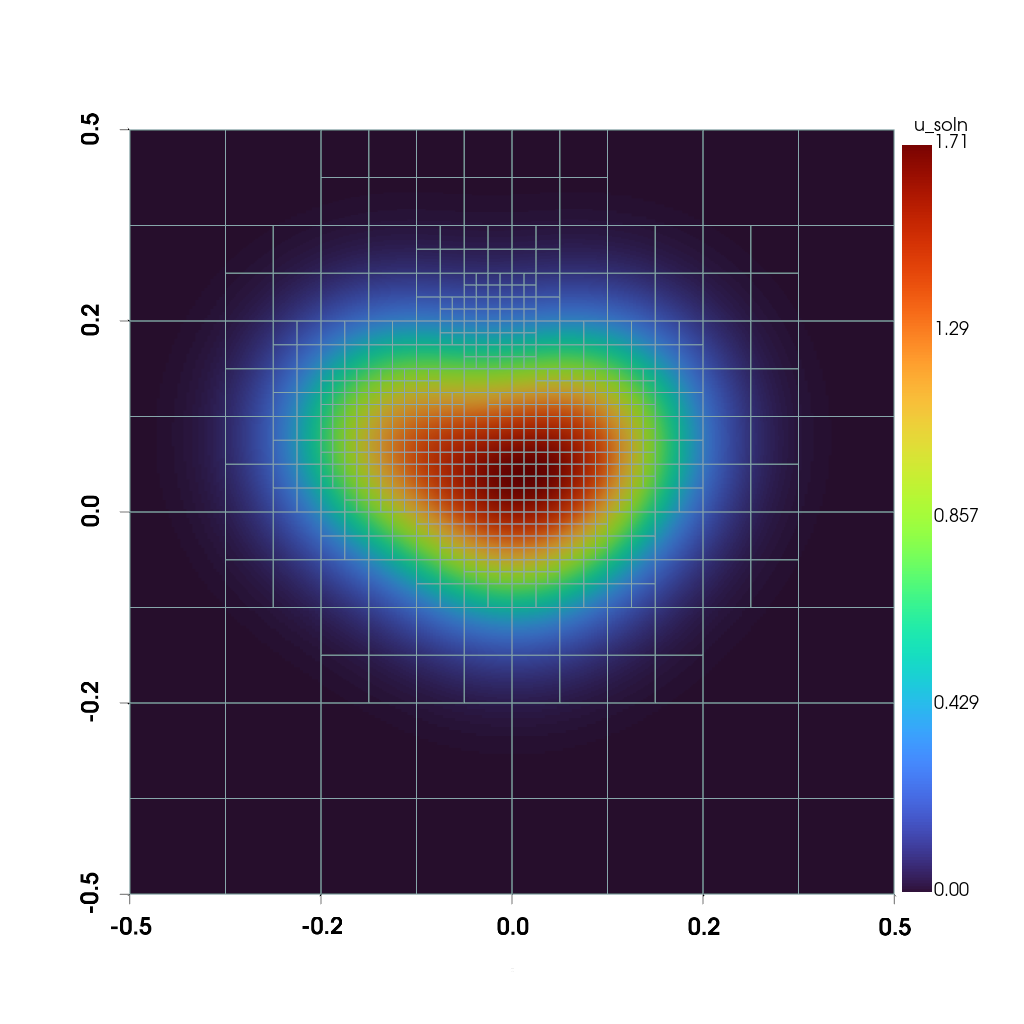
\includegraphics[width=\textwidth, clip=true, trim={0 80 0 0}]{figures/plot_helmholtz_u.png}
%         \end{subfigure}
%         &
%         \begin{subfigure}[t]{0.46\textwidth}
%             \centering
%             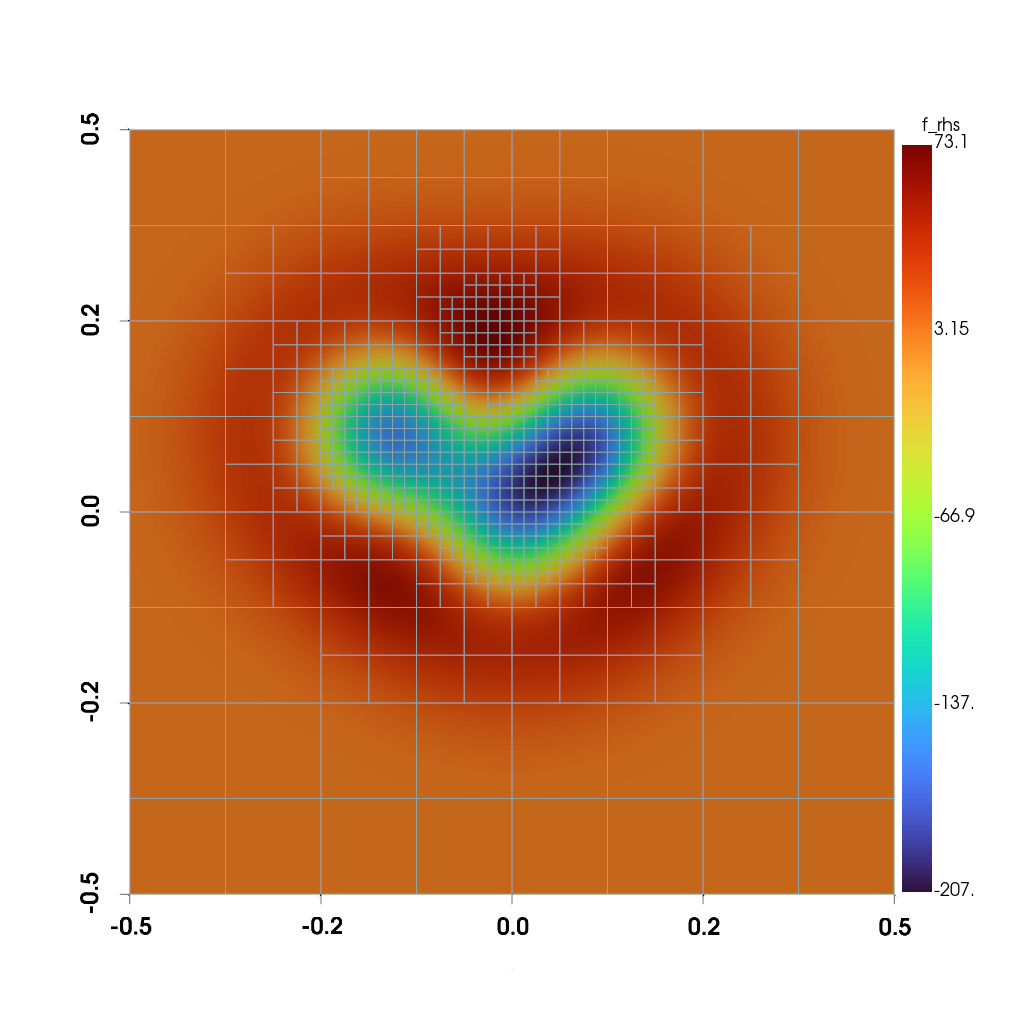
\includegraphics[width=\textwidth, clip=true, trim={0 80 0 0}]{figures/plot_helmholtz_f.png}
%         \end{subfigure}
%     \end{tabular}\\
%     \caption{Mesh and plot of Helmholtz's equations. The left plot is the computed solution and the right plot is the right-hand side.}
%     \label{fig:helmholtz_plots}
% \end{figure}

\begin{figure}
    \centering
    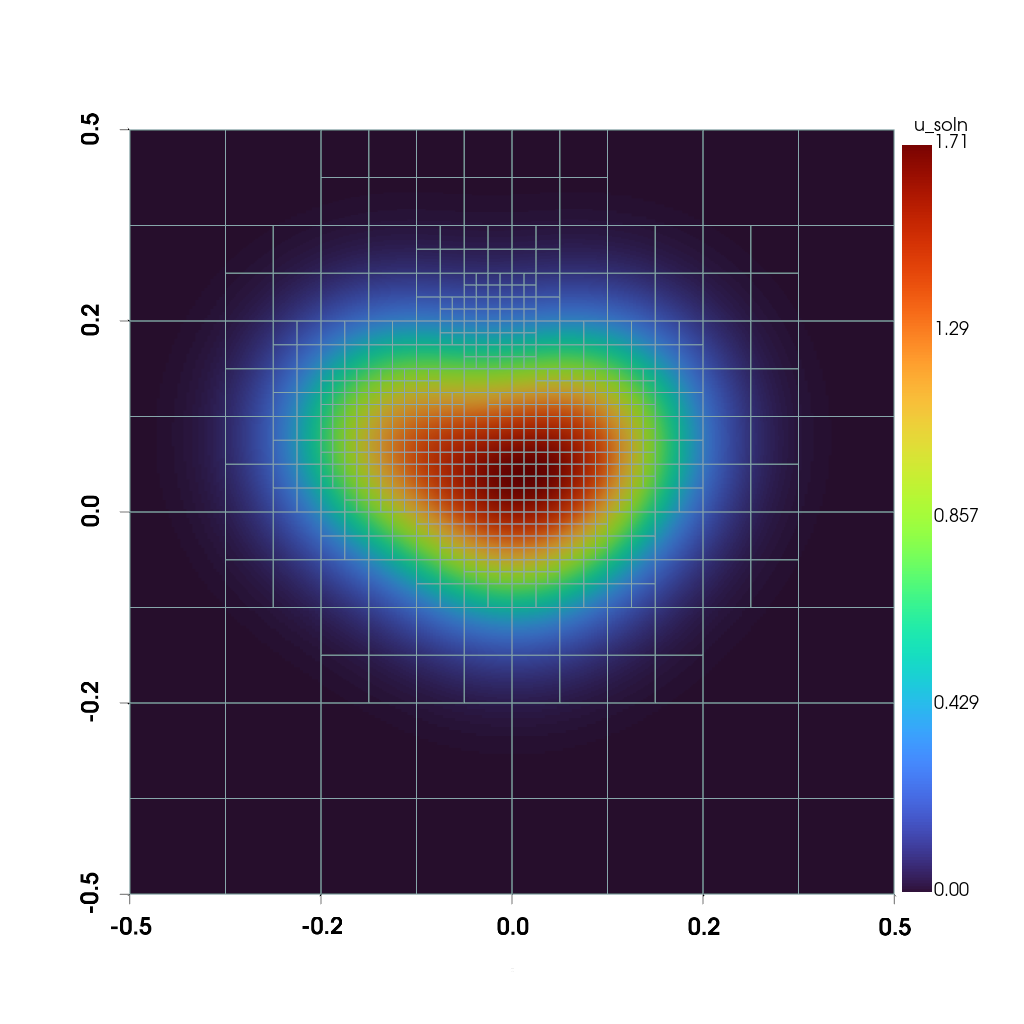
\includegraphics[width=0.75\textwidth, trim={0 100 0 0}]{figures/plot_helmholtz_u.png}
    \caption{Mesh and plot of the solution to the Helmholtz problem in \refsec{sub:helmholtz_equation}.}
    \label{fig:helmholtz_u_plot}
\end{figure}

\begin{figure}
    \centering
    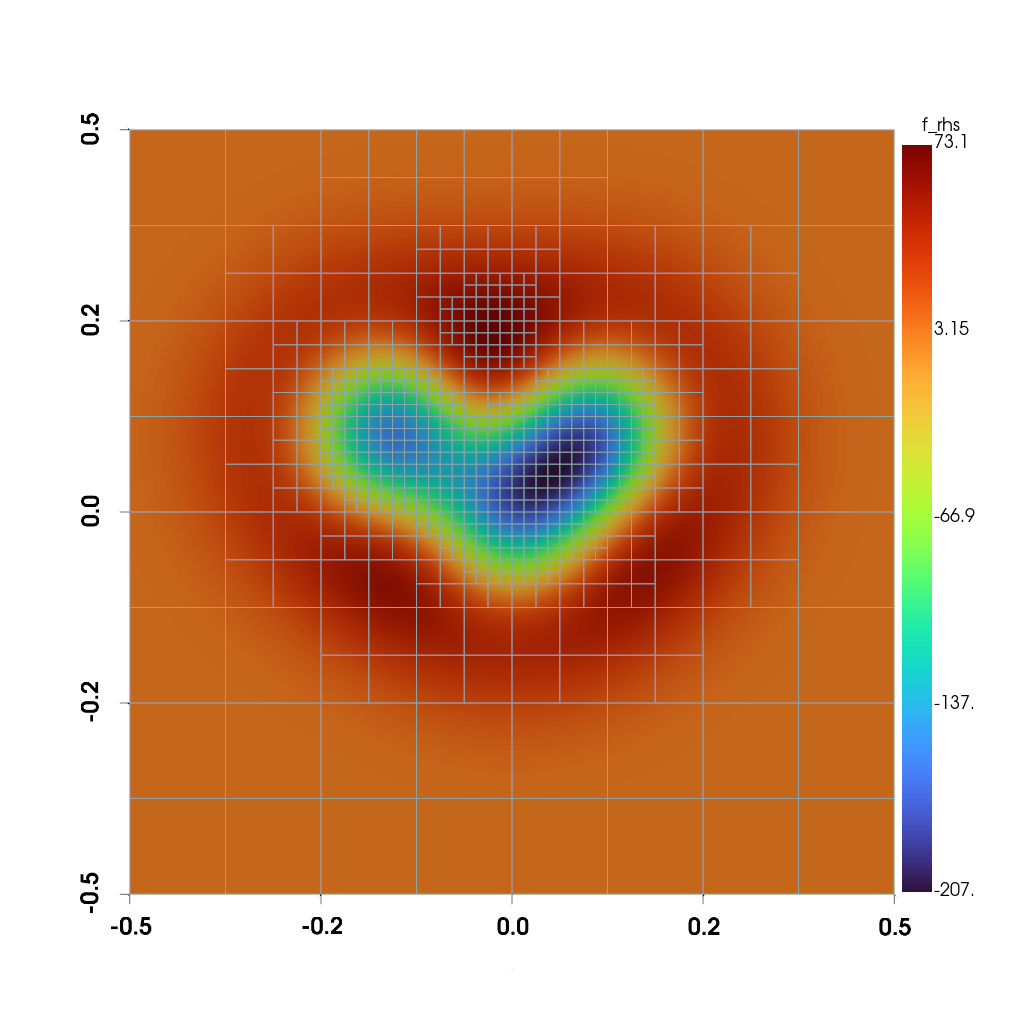
\includegraphics[width=0.75\textwidth, trim={0 100 0 0}]{figures/plot_helmholtz_f.png}
    \caption{Mesh and right-hand side of the solution to the Helmholtz problem in \refsec{sub:helmholtz_equation}.}
    \label{fig:helmholtz_f_plot}
\end{figure}

\begin{table}
    \caption{Convergence analysis for the Helmholtz problem. The upper part shows convergence for a uniformly refined mesh, while the lower part shows convergence for an adaptively refined mesh. $M$ is the size of the grid on each leaf patch, $L_{\text{max}}$ is the maximum level of refinement, $R_{\text{eff}}$ is the effective resolution for a uniformly refined mesh, DOFs is the total degrees of freedom (i.e., total mesh points), $L_{\infty}$ error is the infinity norm error, $L_{\infty}$ order is the infinity norm convergence order, $L_1$ error is the $1^{\text{st}}$ norm error, and $L_1$ order is the $1^{\text{st}}$ norm convergence order.}
    \centering
    \sisetup{
        table-alignment-mode=format
    }
    \begin{tabular}{
        |
        S   % Patch size
        S[table-column-width=0.8cm]   % Max level
        S[table-text-alignment=right, table-column-width=0.7cm]   % Effective resolution
        S[table-text-alignment=right, table-column-width=1.4cm]   % DOFs
        S[scientific-notation=true, round-mode=places, round-precision=2, table-column-width=1.65cm]   % L-inf error
        S[scientific-notation=false, exponent-mode=fixed, round-mode=places, round-precision=2, table-column-width=1.5cm]   % L-inf order
        S[scientific-notation=true, round-mode=places, round-precision=2]   % L-1 error
        S[scientific-notation=false, exponent-mode=fixed, round-mode=places, round-precision=2]   % L-1 order
        |
    }
\hline
{M} & {$L_{\text{max}}$} & {$R_{\text{eff}}$} & {DOFs} & {$L_{\infty}$ Error} & {$L_{\infty}$ Order} & {$L_1$ Error} & {$L_1$ Order} \\
\hline
% \num{16} & \num{1} & \num{32} & \num{1024} & \num{1.29237401760500E-02} & \num{0.00000000000000E+00} & \num{1.41621768661641E-03} & \num{0.00000000000000E+00} \\
% \num{16} & \num{2} & \num{64} & \num{4096} & \num{3.24474376001426E-03} & \num{1.99384719443466E+00} & \num{3.52042103641637E-04} & \num{2.00822315072563E+00} \\
\num{16} & \num{3} & \num{128} & \num{16384} & \num{8.11856103331010E-04} & \num{1.99880860589163E+00} & \num{8.79086298739653E-05} & \num{2.00167127817603E+00} \\
\num{16} & \num{4} & \num{256} & \num{65536} & \num{2.02984786720650E-04} & \num{1.99985243641999E+00} & \num{2.19695214703194E-05} & \num{2.00050135378016E+00} \\
\num{16} & \num{5} & \num{512} & \num{262144} & \num{5.07454266427398E-05} & \num{2.00002189203670E+00} & \num{5.49192113777069E-06} & \num{2.00012063189787E+00} \\
\num{16} & \num{6} & \num{1024} & \num{1048576} & \num{1.26864921798919E-05} & \num{1.99998458881074E+00} & \num{1.37295318659519E-06} & \num{2.00002847405489E+00} \\
\num{16} & \num{7} & \num{2048} & \num{4194304} & \num{3.17161259033582E-06} & \num{2.00000475557083E+00} & \num{3.43237939677034E-07} & \num{2.00000150042016E+00} \\
% \num{32} & \num{1} & \num{64} & \num{4096} & \num{3.24474376001093E-03} & \num{0.00000000000000E+00} & \num{3.52042103642942E-04} & \num{0.00000000000000E+00} \\
% \num{32} & \num{2} & \num{128} & \num{16384} & \num{8.11856103339447E-04} & \num{1.99880860587515E+00} & \num{8.79086298732444E-05} & \num{2.00167127819321E+00} \\
\num{32} & \num{3} & \num{256} & \num{65536} & \num{2.02984786837223E-04} & \num{1.99985243560645E+00} & \num{2.19695214601884E-05} & \num{2.00050135443361E+00} \\
\num{32} & \num{4} & \num{512} & \num{262144} & \num{5.07454269149665E-05} & \num{2.00002188512581E+00} & \num{5.49192111200352E-06} & \num{2.00012063800147E+00} \\
\num{32} & \num{5} & \num{1024} & \num{1048576} & \num{1.26864947160854E-05} & \num{1.99998430813683E+00} & \num{1.37295295907976E-06} & \num{2.00002870635855E+00} \\
\num{32} & \num{6} & \num{2048} & \num{4194304} & \num{3.17160773866120E-06} & \num{2.00000725090321E+00} & \num{3.43238375314458E-07} & \num{1.99999943028095E+00} \\
\hline
% \num{16} & \num{1} & \num{32} & \num{1024} & \num{1.29237401760500E-02} & \num{0.00000000000000E+00} & \num{1.41621768661641E-03} & \num{0.00000000000000E+00} \\
% \num{16} & \num{2} & \num{64} & \num{4096} & \num{3.24474376001426E-03} & \num{1.99384719443466E+00} & \num{3.52042103641637E-04} & \num{2.00822315072563E+00} \\
\num{16} & \num{3} & \num{128} & \num{8704} & \num{1.35786298229745E-03} & \num{1.25676664286521E+00} & \num{1.62110560935590E-04} & \num{1.11876990262527E+00} \\
\num{16} & \num{4} & \num{256} & \num{22528} & \num{1.64905762929112E-03} & \num{-2.80303908147837E-01} & \num{8.45781698947318E-05} & \num{9.38620831715358E-01} \\
\num{16} & \num{5} & \num{512} & \num{54784} & \num{2.38573635354355E-03} & \num{-5.32792803144748E-01} & \num{3.38667165953099E-05} & \num{1.32041722042279E+00} \\
\num{16} & \num{6} & \num{1024} & \num{163072} & \num{5.94628321314072E-04} & \num{2.00437453684095E+00} & \num{1.31283531083692E-05} & \num{1.36718217508683E+00} \\
\num{16} & \num{7} & \num{2048} & \num{485632} & \num{7.32427776781507E-04} & \num{-3.00698326888675E-01} & \num{1.91363184831188E-05} & \num{-5.43627357312482E-01} \\
% \num{32} & \num{1} & \num{64} & \num{4096} & \num{3.24474376001093E-03} & \num{0.00000000000000E+00} & \num{3.52042103642942E-04} & \num{0.00000000000000E+00} \\
% \num{32} & \num{2} & \num{128} & \num{16384} & \num{8.11856103339447E-04} & \num{1.99880860587515E+00} & \num{8.79086298732444E-05} & \num{2.00167127819321E+00} \\
\num{32} & \num{3} & \num{256} & \num{34816} & \num{3.39042440507864E-04} & \num{1.25975816324197E+00} & \num{4.06849021440135E-05} & \num{1.11151127906479E+00} \\
\num{32} & \num{4} & \num{512} & \num{90112} & \num{4.02109898754332E-04} & \num{-2.46123973731869E-01} & \num{2.13036585418219E-05} & \num{9.33392310591107E-01} \\
\num{32} & \num{5} & \num{1024} & \num{222208} & \num{5.85657916098325E-04} & \num{-5.42468378289773E-01} & \num{8.31054203108411E-06} & \num{1.35808672932660E+00} \\
\num{32} & \num{6} & \num{2048} & \num{664576} & \num{1.50576960741055E-04} & \num{1.95955718461569E+00} & \num{3.71801364039699E-06} & \num{1.16041051254945E+00} \\
\hline
    \end{tabular}
    \label{tab:helmholtz_results}
\end{table}

\begin{table}
    \caption{Timing and memory results for the Helmholtz problem. The upper part shows results for the uniformly refined mesh, while the lower part shows results for the adaptively refined mesh. The results here are for a patch size of $16 \times 16$. $L_{\text{max}}$ is the maximum level of refinement, $R_{\text{eff}}$ is the effective resolution, DOFs is the total degrees of freedom, $T_{\text{build}}$ is the time in seconds for the build stage, $T_{\text{upwards}}$ is the time in seconds for the upwards stage, $T_{\text{solve}}$ is the time in seconds for the solve stage, and $S$ is the memory storage in megabytes to store the quadtree and all data matrices stored in each node of the quadtree.}
    \centering
    \sisetup{
        table-alignment-mode=format
    }
    \begin{tabular}{
        |
        S[table-column-width=0.8cm]   % Max level
        S[table-text-alignment=right, table-column-width=0.7cm]   % Effective resolution
        S[table-text-alignment=right, table-column-width=1.4cm]   % DOFs
        S[table-text-alignment=right, scientific-notation=false, exponent-mode=fixed, round-mode=places, round-precision=2]   % Build time
        S[table-text-alignment=right, scientific-notation=false, exponent-mode=fixed, round-mode=places, round-precision=2]   % Upwards time
        S[table-text-alignment=right, scientific-notation=false, exponent-mode=fixed, round-mode=places, round-precision=2]   % Solve time
        S[table-text-alignment=right, scientific-notation=false, exponent-mode=fixed, round-mode=places, round-precision=2]   % Memory size
        |
    }
\hline
{$L_{\text{max}}$} & {$R_{\text{eff}}$} & {DOFs} & {$T_{\text{build}}$ (sec)} & {$T_{\text{upwards}}$ (sec)} & {$T_{\text{solve}}$ (sec)} & {$S$ (MB)} \\
\hline
\num{3} & \num{128} & \num{16384} & \num{3.01504249999999E-01} & \num{7.933354200E-02} & \num{4.67959999999999E-02} & \num{1.58822374343872E+01} \\
\num{4} & \num{256} & \num{65536} & \num{1.49072670900000E+00} & \num{3.993616660E-01} & \num{1.95166584000000E-01} & \num{8.15484972000122E+01} \\
\num{5} & \num{512} & \num{262144} & \num{7.21594766700000E+00} & \num{1.882675541E+00} & \num{9.14324582999999E-01} & \num{3.98233067512512E+02} \\
\num{6} & \num{1024} & \num{1048576} & \num{3.38984894589999E+01} & \num{8.795803542E+00} & \num{3.89846425000000E+00} & \num{1.88101041126251E+03} \\
\num{7} & \num{2048} & \num{4194304} & \num{1.59021219833999E+02} & \num{4.257397542E+01} & \num{1.88671120829999E+01} & \num{8.67619791126251E+03} \\
\hline
\num{3} & \num{128} & \num{8704} & \num{1.29889625000000E-01} & \num{2.823758300E-02} & \num{1.49769169999999E-02} & \num{4.63061237335205E+00} \\
\num{4} & \num{256} & \num{22528} & \num{3.62822042000000E-01} & \num{8.477891600E-02} & \num{2.33342910000000E-02} & \num{1.33817796707153E+01} \\
\num{5} & \num{512} & \num{54784} & \num{8.70019541999999E-01} & \num{1.982561250E-01} & \num{4.41358329999999E-02} & \num{2.84357728958129E+01} \\
\num{6} & \num{1024} & \num{163072} & \num{2.88925454100000E+00} & \num{7.241970830E-01} & \num{1.29217458000000E-01} & \num{1.16809662818908E+02} \\
\num{7} & \num{2048} & \num{485632} & \num{9.30737075000000E+00} & \num{2.389094875E+00} & \num{3.30502583999999E-01} & \num{3.95934556007385E+02} \\
\hline
    \end{tabular}
    \label{tab:helmholtz_timing}
\end{table}

% \begin{figure}
%     \centering
%     \begin{tabular}{cc}
%         \begin{subfigure}[t]{0.3\textwidth}
%             \centering
%             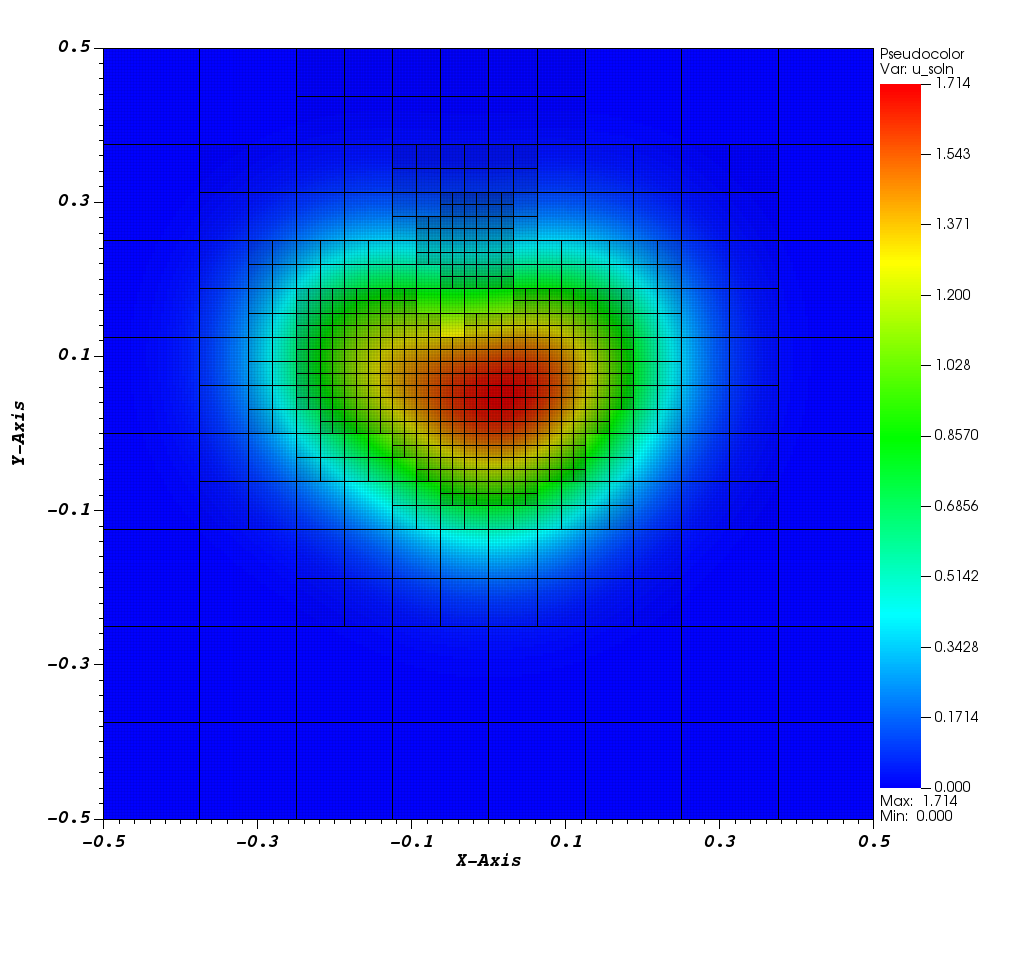
\includegraphics[width=\textwidth]{figures/figure_helmholtz_u.png}
%         \end{subfigure}
%         &
%         \begin{subfigure}[t]{0.3\textwidth}
%             \centering
%             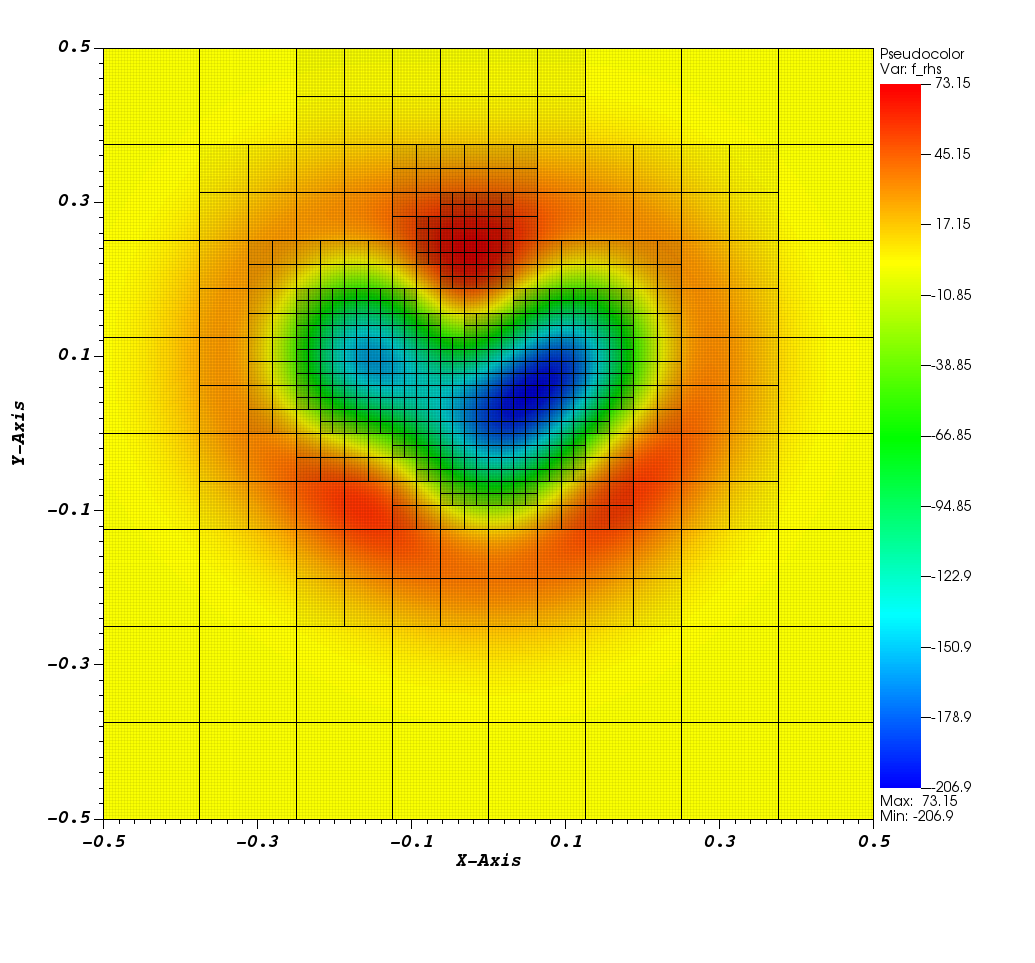
\includegraphics[width=\textwidth]{figures/figure_helmholtz_f.png}
%         \end{subfigure}
%     \end{tabular}
%     \caption{TODO}
%     \label{fig:helmholtz_plots}
% \end{figure}

% \subsection{Laplace's Equation I}

% We solve the following boundary value problem
% \begin{align}
%     \begin{cases}
%         \text{PDE: } & \nabla^2 u(x,y) = 0, (x,y) \in \Omega = [-1, 1] \times [-1 1] \\
%         \text{BC:  } & u(x,y) = g(x,y), (x,y) \in \Gamma = \partial \Omega. \\
%     \end{cases}
%     \label{eqn:laplace}
% \end{align}
% Using a method of manufactured solutions, we compare the numerical solution to an exact solution
% \begin{align}
%     u_{exact}(x,y) = \sin(2 \pi x) \sinh(2 \pi y).
% \end{align}

% \donna{say what $g(x,y)$ is. }

% \donna{It would be great to have a plot here.  Maybe both uniform and adaptive plots?}

% \ignore{As this is a homogeneous problem, there will be no refinement based on the right-hand side.} This acts as an initial test to make sure that the merging and splitting algorithms detailed above are consistent with the order of the patch solver. Using the FISHPACK90 patch solver, we should expect $2^{nd}$ order convergence \citep{adams2016fishpack90}. \donna{Describe the FV discretization.  Fishpack is just a way to solve the resulting linear algebra problem.}

% We solve \ignore{Laplace's equation}  by creating the uniform mesh up to a specified level of refinement $L$. Each patch consists of an $M \times M$ grid of cell-centered points. \donna{Have you described the finite volume discretization?}.  \ignore{The effective resolution $R_{eff}$ is the number of cell-centered points along an entire side of the domain for a uniformly refined mesh.} \ignore{The effective resolution is computed as $R_{eff} = \{\text{Number of patches per side}\} \times \{\text{Number of points per patch}\} = 2^{L+1} \times M$.} We define {\em effective resolution} as $R_{\mbox{eff}}M 2^L$. \donna{Double check this formula.  You probably don't need to spell out in words.}.  For the uniform case, there are several ways to get the same effective resolution. 

% For example, $512 = 8 \times 2^6 = 16 \times 2^5 32 \times 2^4$ and so on. 

% \ignore{For example, on a uniform mesh, to get a $512 \times 512$ resolution, one could use a quadtree with 1 level of refinement (yielding a 2x2 grid of patches) with a patch size of 256x256, or a quadtree with 2 levels of refinement (yielding a 4x4 grid of patches) with a patch size of 128x128, or a quadtree with 3 levels of refinement (yielding an 8x8 grid of patches) with a patch size of 64x64.} 

% \donna{You can,also create an artificial refinement - i.e. refine along diagonals, or something.}

% \subsubsection{Results and Analysis}

% For a given effective resolution, we have observed that the error is essentially independent of the manner in which we achieve the effective resolution.  

%  the same on a uniform grid. Thus, in the subsequent tables, only the effective resolution is shown, despite having run several additional parameter sweeps.  \donna{What do you mean by parameter sweep here?}

% \donna{use siunitx}


% %$ $\begin{center}
% %$ $\sisetup{detect-weight=true,detect-inline-weight=math}
% %$ $\begin{tabular}{
% %$ $   S[table-text-alignment=right]
% %$ $  *2{S[table-column-width=2.25cm,
% %$ $       table-format=2.2e10,
% %$ $       scientific-notation=true,                  
% %$ $       round-mode=places,round-precision=2]}
% %$ $}  % end of column definition
% %$ $\toprule
% %$ $ & \multicolumn{1}{m{2cm}}{\centering Conservation error} &
% %$ $\multicolumn{1}{m{2cm}}{\centering $\infty$-norm error} \\
% %$ $\midrule 
% %$ ${No correction}          & \num{2.4764404912458460e-04} &  \num{1.2338e-01}\\
% %$ ${Fluctuation correction} & \num{2.5302713046460035e-05} &  \num{9.3793e-02}\\
% %$ ${Flux correction}        & \num{2.5111614390205261e-04} &  \num{1.2293e-01}\\
% %$ ${All corrections}        & \num{0.0000000000000000e+00} &  \num{9.5006e-02}\\
% %$ $\bottomrule
% %$ $\end{tabular}
% %$ $\end{center}
% %$ $\label{tab:conservation_cubedsphere}
% %$ $\end{table}

% % Table generated by Excel2LaTeX from sheet 'laplace-1'
% \begin{table}[htbp]
%     \centering
%     \caption{Convergence and Timing for the Laplace I Problem. The columns show the effective resolution $R_{eff}$, the $L_1$ error computed from the exact solution, the order of convergence, timing for the build $T_{build}$ and solve $T_{solve}$ stages, and the required memory $S$ to store the factorization. The data show expected second order convergence.   \donna{Is data for a fixed patch size? Add a column for the level used.}}
%     \begin{tabular}{|r|r|r|r|r|r|}
%         \toprule
%         \multicolumn{1}{|l|}{$R_{eff}$} & \multicolumn{1}{l|}{$L_1$ Error} & \multicolumn{1}{l|}{Order} & \multicolumn{1}{l|}{$T_{build}$ (sec)} & \multicolumn{1}{l|}{$T_{solve}$ (sec)} & \multicolumn{1}{l|}{S (MB)} \\
%         \midrule
%         \midrule
%         8     & 3.0580E+00 &       & 2.3421E-04 & 1.0308E-03 & 9.2936E-03 \\
%         16    & 1.0991E+00 & 1.4762E+00 & 1.0122E-03 & 9.1642E-04 & 3.6149E-02 \\
%         32    & 3.0879E-01 & 1.8317E+00 & 7.6679E-03 & 5.4845E-03 & 1.4259E-01 \\
%         64    & 7.9664E-02 & 1.9546E+00 & 5.4575E-02 & 1.8398E-02 & 5.6642E-01 \\
%         128   & 2.0097E-02 & 1.9869E+00 & 4.6770E-01 & 5.7012E-02 & 2.2578E+00 \\
%         256   & 5.0345E-03 & 1.9971E+00 & 2.1628E+00 & 2.1096E-01 & 2.7051E+01 \\
%         512   & 1.2594E-03 & 1.9991E+00 & 9.8592E+00 & 9.1265E-01 & 1.8024E+02 \\
%         1024  & 3.1488E-04 & 1.9998E+00 & 4.4384E+01 & 3.9901E+00 & 1.0090E+03 \\
%         2048  & 7.8723E-05 & 2.0000E+00 & 1.9991E+02 & 1.8425E+01 & 5.1883E+03 \\
%         \bottomrule
%     \end{tabular}%
%     \label{tab:laplace-1}%
% \end{table}%

% \donna{Try with more levels. }


% As \reftab{tab:laplace-1} shows, our current implementations shows the expected second order convergence.   The merging and splitting algorithms detailed in this paper are consistent with the order of the patch solver. \donna{These results are consistent with the results shown in M and G.  The linear algebra involved in merging and splitting does not causes errors to propagate}.  The timing for the build and solve stages grow as the resolution grows. Storage for the set of solution operators also grows as the resolution increases. 

% Direct methods tend to be more storage intensive than iterative methods. The adaptive implementation will help decrease the memory requirements for the HPS method. \donna{This is a better statement for the conclusions, since it is a very general statement. }

% \subsection{Poisson's Equation I}

% We solve the following boundary value problem
% \begin{align}
%     \begin{cases}
%         \text{PDE: } & \nabla^2 u(x,y) = f(x,y), (x,y) \in \Omega = [-1, 1] \times [-1 1] \\
%         \text{BC:  } & u(x,y) = g(x,y), (x,y) \in \Gamma = \partial \Omega. \\
%     \end{cases}
% \end{align}
% with a manufactured exact solution of
% \begin{align}
%     u_{exact}(x,y) &= \sin(c \pi x) + \cos(c \pi y) \\
%     f(x,y) &= -(c \pi)^2 u(x,y).
% \end{align}
% We use $c = 2$ for this case.

% With an inhomogeneous right-hand side, we can adapt the mesh according to the load function $f$. Where $|f(x,y)|$ is large, the curvature of the solution is large. Thus, we refine according to $|f(x,y)| > \epsilon$, with $\epsilon = 50$ for this case.

% \subsubsection{Results and Analysis}

% The results of this convergence study are shown in \reftab{tab:poisson-1}. As in the first example, we report the error with increasing effective resolution. The upwards time reported in \reftab{tab:poisson-1} shows the time required for the upwards pass needed with a non-homogeneous elliptic problem as outlined in \refsec{subsub:4to1-upwards}.

% % Table generated by Excel2LaTeX from sheet 'poisson-1'
% \begin{table}[htbp]
%     \centering
%     \begin{tabular}{|r|r|r|r|r|r|}
%         \toprule
%         \multicolumn{1}{|l|}{$R_{eff}$} & \multicolumn{1}{l|}{$L_{1}$ Error} & \multicolumn{1}{l|}{Order} & \multicolumn{1}{l|}{$T_{build}$ (sec)} & \multicolumn{1}{l|}{$T_{upwards}$ (sec)} & \multicolumn{1}{l|}{$T_{solve}$ (sec)} \\
%         \midrule
%         64    & 2.55E-03 &       & 5.41E-02 & 7.19E-03 & 2.46E-02 \\
%         128   & 6.36E-04 & 2.00E+00 & 2.77E-01 & 5.60E-02 & 7.04E-02 \\
%         256   & 1.59E-04 & 2.00E+00 & 1.49E+00 & 2.95E-01 & 2.26E-01 \\
%         512   & 7.37E-05 & 1.11E+00 & 3.52E+00 & 5.58E-01 & 2.87E-01 \\
%         1024  & 1.86E-05 & 1.99E+00 & 1.60E+01 & 3.26E+00 & 1.24E+00 \\
%         \midrule
%         128   & 6.36E-04 &       & 2.98E-01 & 2.95E-02 & 5.12E-02 \\
%         256   & 1.59E-04 & 2.00E+00 & 1.51E+00 & 2.15E-01 & 2.11E-01 \\
%         512   & 3.97E-05 & 2.00E+00 & 7.29E+00 & 1.11E+00 & 9.49E-01 \\
%         1024  & 1.86E-05 & 1.09E+00 & 1.60E+01 & 2.05E+00 & 1.18E+00 \\
%         2048  & 4.67E-06 & 1.99E+00 & 7.58E+01 & 1.16E+01 & 5.44E+00 \\
%         \bottomrule
%     \end{tabular}%
%     \caption{Convergence and Timing for the Poisson I Problem. The columns report the effective resolution $R_{eff}$, the $L_1$ error, the order of convergence, and the timing for the build $T_{build}$, upwards $T_{upwards}$, and $T_{solve}$ stages.}
%     \label{tab:poisson-1}%
% \end{table}%  

% This numerical experiment shows that even with an adaptive scheme, we maintain the expected $2^{nd}$ order convergence. The timing for the build and solve stages is also faster than the build and solve stages of the Laplace example, almost by an order of magnitude.

% \subsection{Poisson's Equation II}

% As another test for Poisson's equation, we solve a ``polar star'' Poisson problem. The problem is created via a method of manufactured solutions and is engineered to have highly local curvature from the load function. The resulting solution is a collection of polar stars with user specified number of points and radii of curvature. This problem highlights the use of an adaptive mesh to solve the elliptic equation. The exact solution we attempt to reconstruct is the following:
% \begin{align}
%     u(x,y) = \frac{1}{2} \sum_{i=1}^{N} 1 - \tanh \left(\frac{r(x,y)-r_{0,i} \left(r_{1,i} \cos \left(n \theta(x,y)\right)+1\right)}{\epsilon }\right)
% \end{align}
% % Details on the right-hand side and parameters can be found in Appendix \ref{apdx:polar_star_problem}.
% Computing the Laplacian analytically yields the right-hand side to Poisson's equation. Thus, the polar star Poisson problem is defined as follows:
% \begin{align}
%     \nabla^2 u(x,y) = \sum_{i=1}^N -\frac{s_{1,i}(x,y) + s_{2,i}(x, y)}{r(x,y)^2} - s_{3,i}(x,y) + s_{4,i}(x,y)
% \end{align}
% with
% \begin{align*}
%     s_{1,i}(x,y) &= \frac{p(x,y)^2 \tanh \left(\phi(x,y)\right) \text{sech}^2\left(\phi(x,y)\right)}{\epsilon ^2} \\
%     s_{2,i}(x,y) &= -\frac{n^2 r_{0,i} r_{1,i} \cos (n \theta(x,y)) \text{sech}^2\left(\phi(x,y)\right)}{2 \epsilon } \\
%     s_{3,i}(x,y) &= \frac{\tanh \left(\phi(x,y)\right) \text{sech}^2\left(\phi(x,y)\right)}{\epsilon ^2} \\
%     s_{4,i}(x,y) &= \frac{\text{sech}^2\left(\phi(x,y)\right)}{2 r(x,y) \epsilon } \\
%     p(x,y) &= n r_{0,i} r_{1,i} \sin (n \theta(x,y)) \\
%     \phi(x,y) &= \frac{r(x,y)-r_{0,i} (r_{1,i} \cos (n \theta(x,y))+1)}{\epsilon}
% \end{align*}
% and where $i=1, ..., N_{polar}$ and $N_{polar}$ is the number of polar stars. Each polar star has a center $(x_0, y_0)$, inner and outer radii $r_0, r_1$, and the number of arms per polar star $n$. The radius and angle have the standard polar transforms:
% \begin{align}
%     r(x,y) &= \sqrt{(x - x_0)^2 + (y - y_0)^2} \\
%     \theta(x,y) &= \tan^{-1}\Big(\frac{y - y_0}{x - x_0}\Big)
% \end{align}
% \reftab{table:polar_star_parameters} has the parameters used in this case study.
% \begin{table}[h]
%     \begin{center}
%         \begin{tabular}{|c|c|c|c|c|c|}
%             \hline
%             $i$ & $x_0$ & $y_0$ & $r_0$ & $r_1$ & $n$ \\
%             \hline
%             $1$ & $-0.5$ & $-0.5$ & $0.1$ & $0.2$ & $4$ \\
%             $2$ & $0.5$ & $0.5$ & $0.1$ & $0.2$ & $7$ \\
%             \hline
%         \end{tabular}
%         \caption{Polar Star Poisson Problem Parameters}
%         \label{table:polar_star_parameters}
%     \end{center}
% \end{table}

% % \begin{figure}
% %     \centering
% %     \begin{tabular}{c c}
% %         \begin{subfigure}[t]{0.45\textwidth}
% %             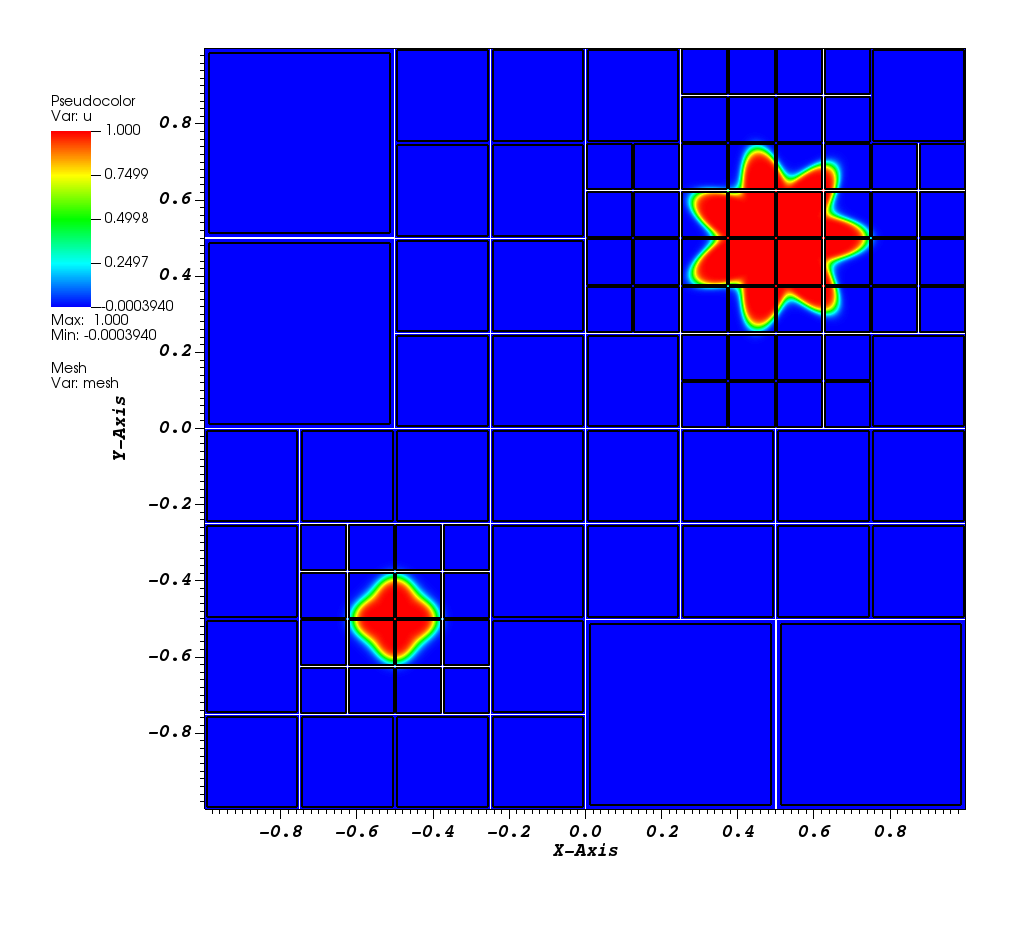
\includegraphics[width=\textwidth]{figures/poisson_2d_solution0000.png}
% %             \caption{Solution}
% %         \end{subfigure}
% %         &
% %         \begin{subfigure}[t]{0.45\textwidth}
% %             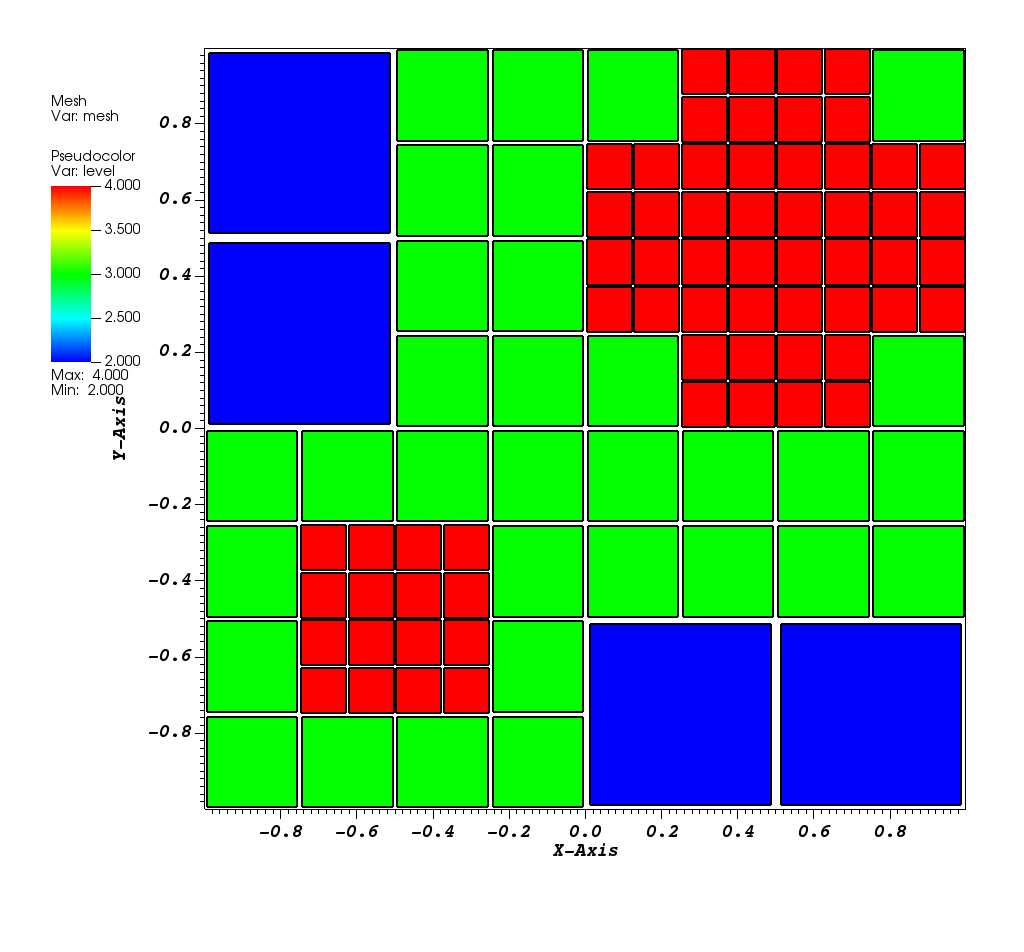
\includegraphics[width=\textwidth]{figures/poisson_levels0000.png}
% %             \caption{Mesh colored by refinement level}
% %         \end{subfigure}
% %     \end{tabular}
% %     \caption{The solution and mesh for the polar star Poisson problem.}
% %     \label{solution_and_mesh_polar_star}
% % \end{figure}

% \subsubsection{Results and Analysis}

% To run a convergence analysis, we solve the polar star Poisson problem on both uniform and adaptive meshes at various resolutions with different patch sizes.

% % Table generated by Excel2LaTeX from sheet 'poisson-2-prev'
% \begin{table}[htbp]
%     \centering
%     \begin{tabular}{|c|c|c|r|r|r|r|r|}
%         \toprule
%         \multicolumn{1}{|l|}{$M$} & \multicolumn{1}{l|}{Mode} & \multicolumn{1}{l|}{$L_{max}$} & \multicolumn{1}{l|}{$R_{eff}$} & \multicolumn{1}{l|}{$N_{DOF}$} & \multicolumn{1}{l|}{$L_1$ Error} & \multicolumn{1}{l|}{Ratio} & \multicolumn{1}{l|}{S (MB)} \\
%         \midrule
%         \midrule
%         \multirow{8}[4]{*}{32} & \multirow{4}[2]{*}{Uniform} & 1     & 64    & 4096  & 1.9397E+00 &       & 1.7003 \\
%         &       & 2     & 128   & 16384 & 4.6616E-01 &       & 11.3109 \\
%         &       & 3     & 256   & 65536 & 2.7698E-02 &       & 63.2631 \\
%         &       & 4     & 512   & 262144 & 1.4022E-04 &       & 325.0915 \\
%         \cmidrule{2-8}          & \multirow{4}[2]{*}{Adaptive} & 1     & 64    & 4096  & 1.9397E+00 & 1.00  & 1.7003 \\
%         &       & 2     & 128   & 10240 & 4.6615E-01 & 0.63  & 4.0637 \\
%         &       & 3     & 256   & 40960 & 2.7698E-02 & 0.63  & 27.5282 \\
%         &       & 4     & 512   & 102400 & 1.3903E-04 & 0.39  & 51.1623 \\
%         \midrule
%         \multirow{8}[4]{*}{64} & \multirow{4}[2]{*}{Uniform} & 1     & 128   & 16384 & 4.6616E-01 &       & 6.7755 \\
%         &       & 2     & 256   & 65536 & 2.7698E-02 &       & 45.1214 \\
%         &       & 3     & 512   & 262144 & 1.4022E-04 &       & 252.5248 \\
%         &       & 4     & 1024  & 1048576 & 2.1169E-05 &       & 1298.1774 \\
%         \cmidrule{2-8}          & \multirow{4}[2]{*}{Adaptive} & 1     & 128   & 16384 & 4.6616E-01 & 1.00  & 6.7755 \\
%         &       & 2     & 256   & 40960 & 2.7698E-02 & 0.63  & 16.1897 \\
%         &       & 3     & 512   & 163840 & 1.4022E-04 & 0.63  & 109.8055 \\
%         &       & 4     & 1024  & 409600 & 2.2336E-05 & 0.39  & 203.9475 \\
%         \midrule
%         \multirow{8}[4]{*}{128} & \multirow{4}[2]{*}{Uniform} & 1     & 256   & 65536 & 2.7698E-02 &       & 27.0509 \\
%         &       & 2     & 512   & 262144 & 1.4022E-04 &       & 180.2425 \\
%         &       & 3     & 1024  & 1048576 & 2.1169E-05 &       & 1009.0483 \\
%         &       & 4     & 2048  & 4194304 & 5.3546E-06 &       & 5188.3493 \\
%         \cmidrule{2-8}          & \multirow{4}[2]{*}{Adaptive} & 1     & 256   & 65536 & 2.7698E-02 & 1.00  & 27.0509 \\
%         &       & 2     & 512   & 163840 & 1.4022E-04 & 0.63  & 64.6291 \\
%         &       & 3     & 1024  & 655360 & 2.1169E-05 & 0.63  & 438.6102 \\
%         &       & 4     & 2048  & 1638400 & 5.6348E-06 & 0.39  & 814.3928 \\
%         \bottomrule
%     \end{tabular}%
%     \caption{Convergence Results for the Poisson II Problem. The columns report the patch size $M$, the mode of mesh generation (uniform or adaptive), the maximum level of refinement $L_{max}$, the total degrees of freedom $N_{DOF}$, the ratio between adaptive and uniform degrees of freedom, and the size $S$ in MB to store the associated data.}
%     \label{tab:poisson-2}%
% \end{table}%

% Figures \ref{plot:timing} and \ref{plot:work_precision} contain resolution vs. timing and timing vs. error (work-precision) plots for the polar-star Poisson problem. Each plot shows results for the build, upwards, and solve stages of the quadtree-adaptive HPS method.

% In \reffig{plot:timing}, the timing for each of the stages is given for various patch sizes and resolutions for both the uniform and adaptive cases. We observe good scaling of the build stage, consistent with the $\mathcal{O}^{3/2}$ scaling of the HPS method. The upwards stage is about an order of magnitude faster than the build stage, and the solve stage is an additional order of magnitude faster. In a transient implementation of this method on a static mesh, the overhead associated with the build stage is outweighed by the time saving of a very fast solve stage each time step. Also note that improvements in timing when using an adaptive scheme. This is shown more in the work-precision plots of \reffig{plot:work_precision}. For the same error, the adaptive implementation can solve the problem $20\%-50\%$ faster.

% \begin{figure}[htbp]
%     \centering
%     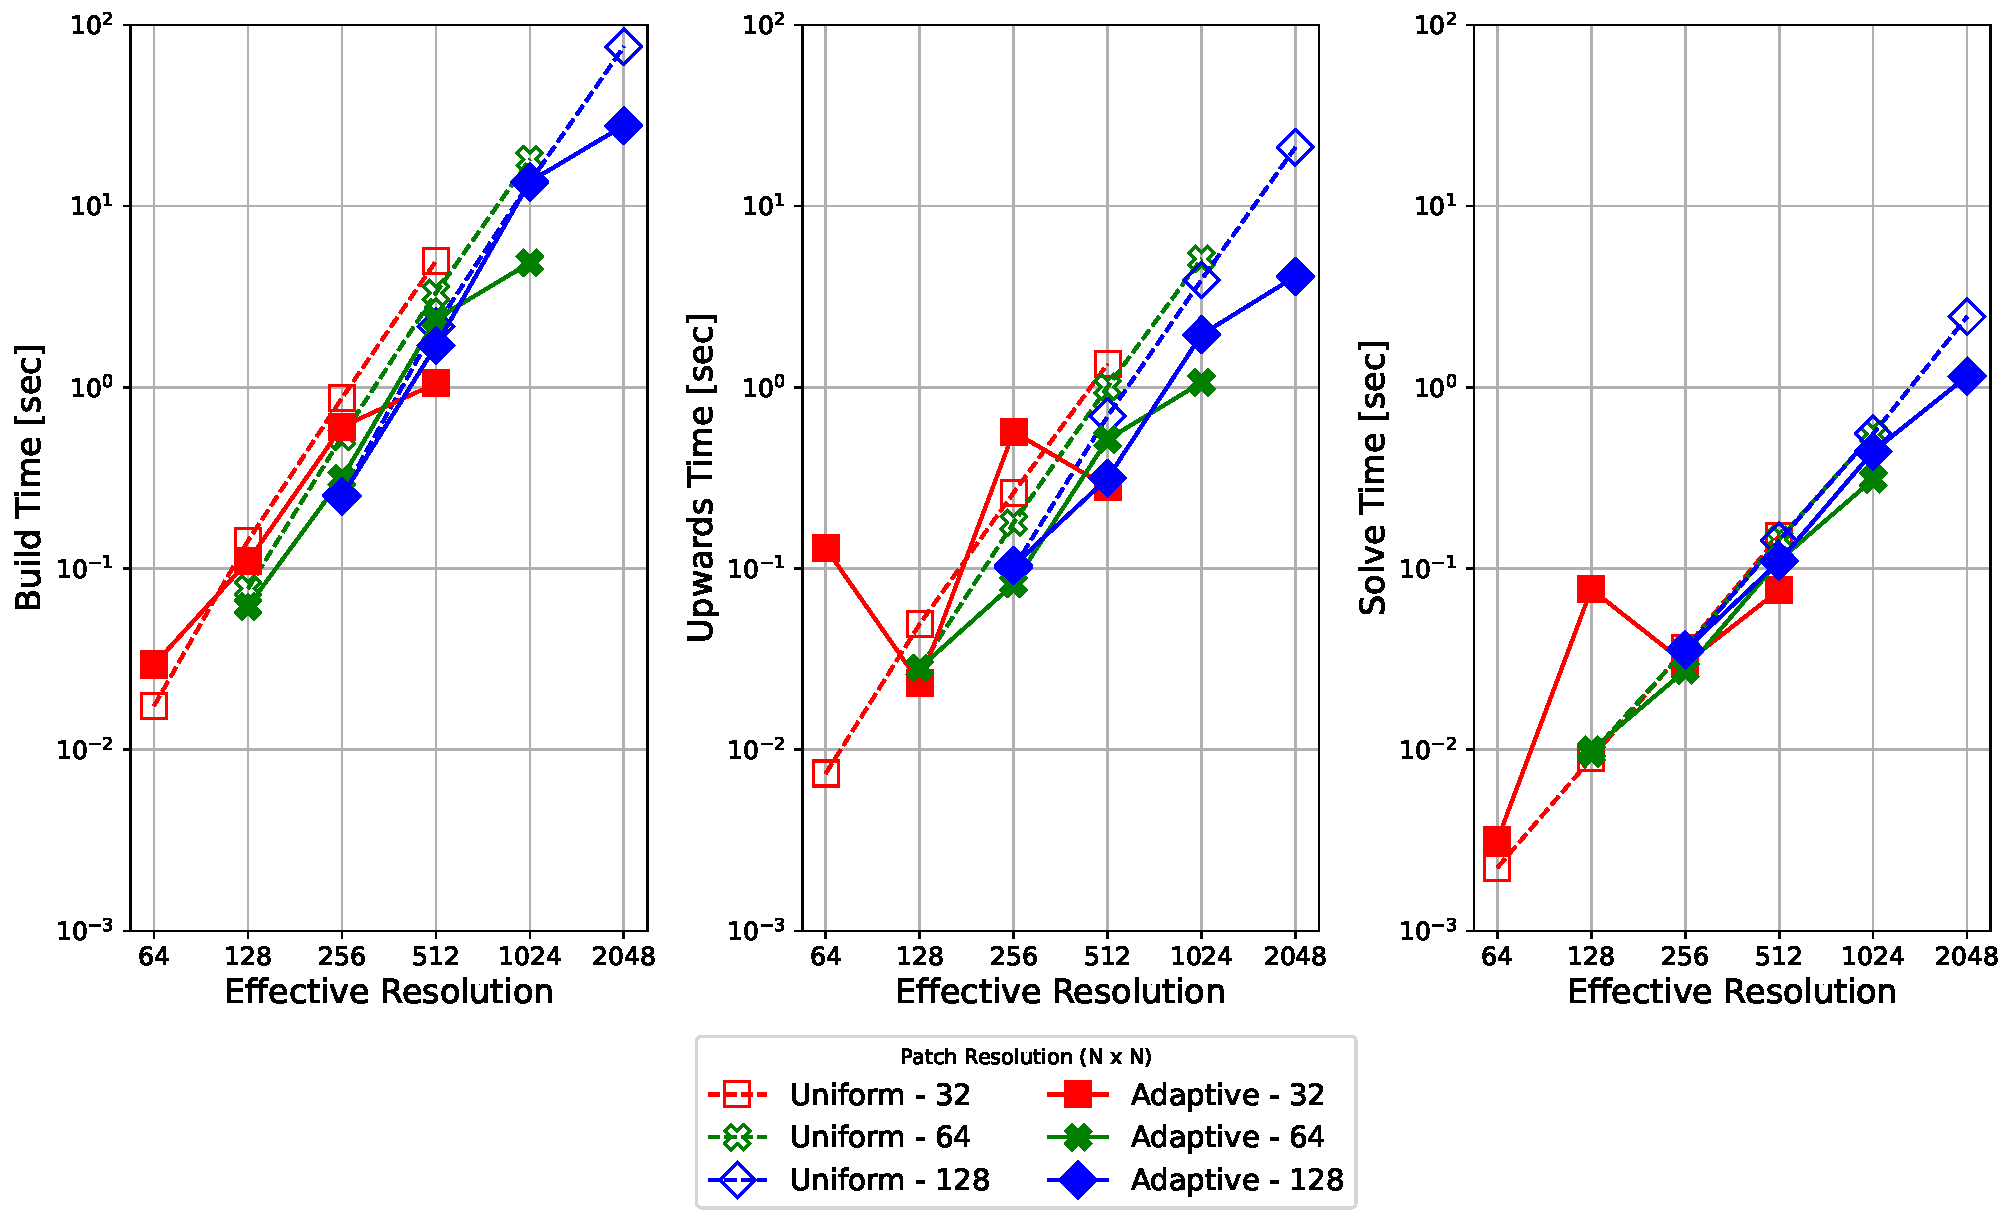
\includegraphics[width=1.0\textwidth]{figures/plot_timing.pdf}
%     \caption{Timing Plots for the Polar-Star Poisson Problem}
%     \label{plot:timing}
% \end{figure}

% \begin{figure}[htbp]
%     \centering
%     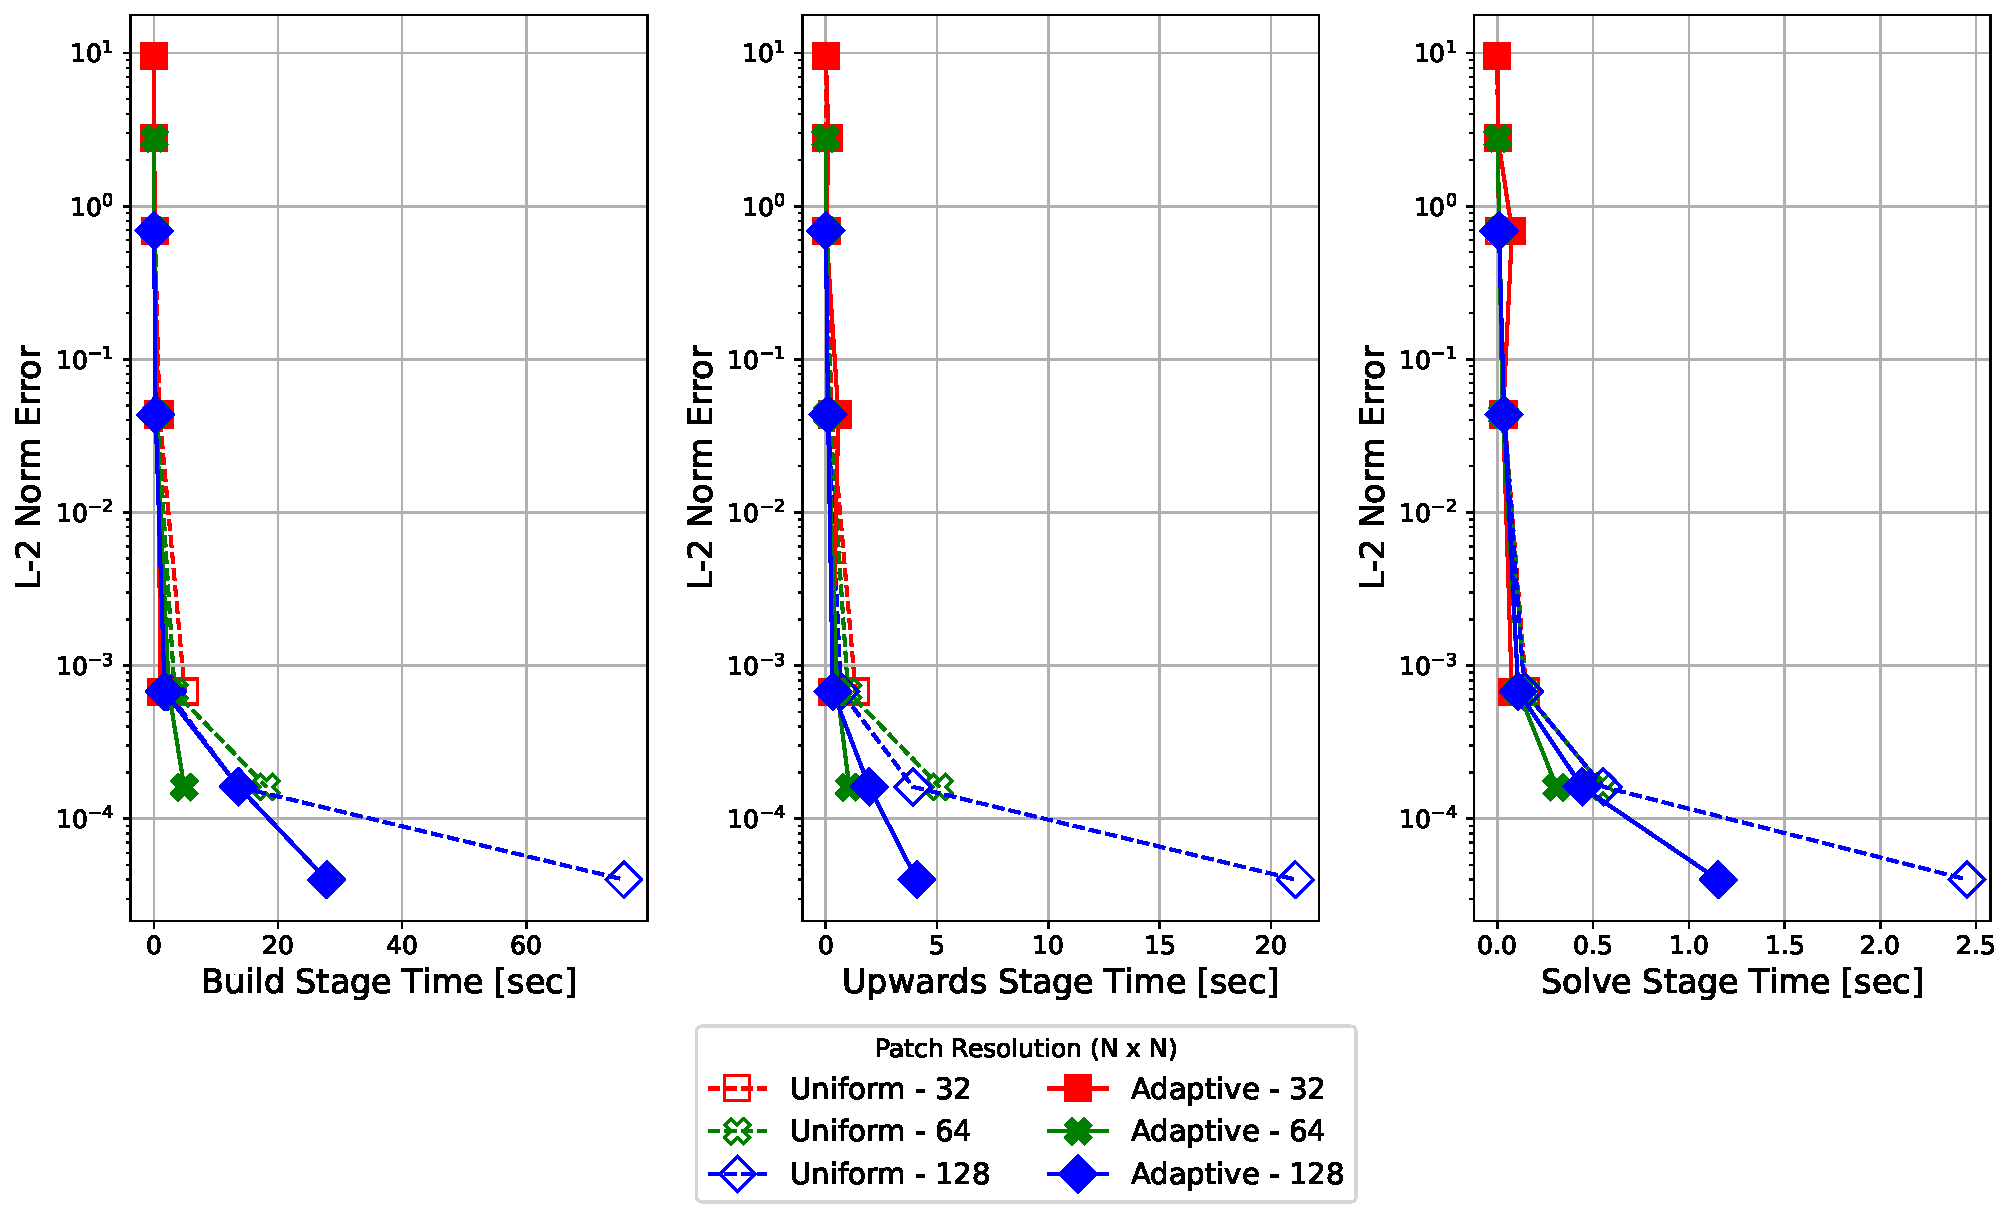
\includegraphics[width=1.0\textwidth]{figures/plot_work_precision.pdf}
%     \caption{Work-Precision Plots for the Polar-Star Poisson Problem}
%     \label{plot:work_precision}
% \end{figure}

% \subsection{Helmholtz's Equation II}

% We now solve the following Helmholtz equation:
% \begin{align}
%     \begin{cases}
%         \text{PDE: } & \nabla^2 u(x,y) + \kappa^2 u(x,y) = 0, (x,y) \in \Omega = [-1, 1] \times [-1 1] \\
%         \text{BC:  } & u(x,y) = g(x,y), (x,y) \in \Gamma = \partial \Omega. \\
%     \end{cases}
% \end{align}
% To provide an exact solution to compare to, we use a manufactured exact solution of
% \begin{align}
%     u_{exact}(x,y) = Y_0(\kappa r(x,y))
% \end{align}
% where $Y_0$ is the zeroth Bessel function of the second kind, $\kappa$ is related to the wavelength $\lambda = \frac{2 \pi}{\kappa}$, and $r(x,y) = \sqrt{(x - x_0)^2 + (y - y_0)^2}$ is the distance from the singularity of the Bessel function. This represents a vibration problem on the domain and is the same problem used in \citep{gillman2014direct} to test their implementation. We use $x_0 = -2, y_0 = 0$ and vary $\kappa$ (as detailed in \reftab{tab:helmholtz-1}).

% A Helmholtz equation with a high wave number suffers from the so-called ``pollution problem''. A high wave number corresponds to a highly oscillatory solution that is difficult to be captured with lower mesh resolutions. To ensure our implementation works for decently large wave numbers, we run a convergence study with varying values of $\kappa$ and check convergence. For more details on the pollution problem, see \citep{peterseim2017eliminating} or \citep{dwarka2021pollution}.

% {\bf Results and Analysis}
% \reftab{tab:helmholtz-1} contains the convergence study and parameter sweep for $\kappa$. We vary $\kappa$ and vary the level of refinement and patch size to get various effective resolutions. The values of the wave number $\kappa$ correspond to values of the wavelength $\lambda$ that vary across three orders of magnitude.

% % Table generated by Excel2LaTeX from sheet 'helmholtz-1'
% \begin{table}[htbp]
%     \centering
%     \begin{tabular}{|c|r|r|r|r|r|r|}
%         \toprule
%         \multicolumn{1}{|l|}{$\kappa$} & \multicolumn{1}{l|}{$R_{eff}$} & \multicolumn{1}{l|}{$L_1$ Error} & \multicolumn{1}{l|}{Order} & \multicolumn{1}{l|}{$T_{build}$ (sec)} & \multicolumn{1}{l|}{$T_{solve}$ (sec)} & \multicolumn{1}{l|}{$S$ (MB)} \\
%         \midrule
%         \midrule
%         \multirow{4}[2]{*}{1} & 256   & 2.24E-06 &       & 7.62E-01 & 2.33E-01 & 2.71E+01 \\
%         & 512   & 5.60E-07 & 2.00E+00 & 2.99E+00 & 9.49E-01 & 1.80E+02 \\
%         & 1024  & 1.40E-07 & 2.00E+00 & 1.81E+01 & 4.00E+00 & 1.01E+03 \\
%         & 2048  & 3.50E-08 & 2.00E+00 & 8.68E+01 & 1.84E+01 & 5.19E+03 \\
%         \midrule
%         \multirow{4}[2]{*}{10} & 256   & 3.28E-04 &       & 7.58E-01 & 2.13E-01 & 2.71E+01 \\
%         & 512   & 8.20E-05 & 2.00E+00 & 2.98E+00 & 9.48E-01 & 1.80E+02 \\
%         & 1024  & 2.05E-05 & 2.00E+00 & 1.59E+01 & 4.30E+00 & 1.01E+03 \\
%         & 2048  & 5.13E-06 & 2.00E+00 & 8.61E+01 & 1.78E+01 & 5.19E+03 \\
%         \midrule
%         \multirow{4}[2]{*}{20} & 256   & 2.58E-03 &       & 7.58E-01 & 2.02E-01 & 2.71E+01 \\
%         & 512   & 8.84E-04 & 1.54E+00 & 2.95E+00 & 9.60E-01 & 1.80E+02 \\
%         & 1024  & 2.61E-04 & 1.76E+00 & 1.58E+01 & 3.93E+00 & 1.01E+03 \\
%         & 2048  & 6.86E-05 & 1.93E+00 & 8.94E+01 & 1.81E+01 & 5.19E+03 \\
%         \midrule
%         \multirow{4}[2]{*}{30} & 256   & 7.89E-03 &       & 7.81E-01 & 2.15E-01 & 2.71E+01 \\
%         & 512   & 1.60E-02 & -1.02E+00 & 2.97E+00 & 9.62E-01 & 1.80E+02 \\
%         & 1024  & 8.08E-04 & 4.31E+00 & 1.59E+01 & 3.97E+00 & 1.01E+03 \\
%         & 2048  & 1.76E-04 & 2.20E+00 & 8.49E+01 & 1.83E+01 & 5.19E+03 \\
%         \midrule
%         \multirow{4}[2]{*}{40} & 256   & 2.72E-02 &       & 7.85E-01 & 2.96E-01 & 2.71E+01 \\
%         & 512   & 1.10E-02 & 1.31E+00 & 2.98E+00 & 9.38E-01 & 1.80E+02 \\
%         & 1024  & 1.00E-03 & 3.46E+00 & 1.61E+01 & 4.01E+00 & 1.01E+03 \\
%         & 2048  & 2.31E-04 & 2.11E+00 & 8.46E+01 & 1.83E+01 & 5.19E+03 \\
%         \bottomrule
%     \end{tabular}%
%     \caption{Convergence Study with Increasing Values of $\kappa$. The columns report the value of the wave number $\kappa$, the effective resolution $R_{eff}$, the $L_1$ error, the order of convergence, the timing for the build $T_{build}$ and solve $T_{solve}$ stages, and the memory storage $S$ for the associated data.}
%     \label{tab:helmholtz-1}%
% \end{table}%

% For each value of $\kappa$, we report the expected $2^{nd}$ order convergence. However, for larger values of $\kappa$, the actual error is lower and lower. This is to be expected at the resolutions we have run our study at. For larger and larger values of $\kappa$, even more resolution would be needed to better capture the smaller and smaller wavelengths. The timing results for this problem are consistent with the times reported in the other problems.

% \subsection{Heat Equation I}

% The time-dependent heat equation can be solved with an elliptic solver as implemented in this paper using a backward Euler time stepping scheme. The heat equation is given as
% \begin{align}
%     \frac{\partial u(x,y,t)}{\partial t} &= \nabla^2 u(x,y,t)
% \end{align}
% for $(x,y) \in \Omega$ and $t \in [0, \infty)$. Applying a backward Euler scheme results in the following:
% \begin{align}
%     \nabla^2 u^{n+1} - \lambda u^{n+1} = -\lambda u^{n}
% \end{align}
% with $\lambda = -\frac{1}{\Delta t}$. This results in a Helmholtz-like equation that we can solve with our implemented HPS method. The advantage to using this scheme is we can perform the build stage prior to any time stepping, then do the upwards and solve stages each time step to perform the update. This results in a very fast and efficient scheme for time-dependent problems. Each time step, the right-hand side is updated with the solution at the previous time step.

% For initial conditions, we will use $u_{exact} = u_0(x,y)$ from the Poisson I test problem. We work on a square domain $\Omega = [0, 1] \times [0, 1]$, with homogeneous, Dirichlet boundary conditions. The analytical solution to this problem can be found via separation of variables and provides an exact solution to compare to. The analytical solution is
% \begin{align}
%     u_{exact}(x,y,t) = \sum_{m=1}^{\infty} \sum_{n=1}^{\infty} A_{mn} \sin(k_x x) \sin(k_y y) e^{-(k_x^2 + k_y^2) t}
% \end{align}
% where $k_x = m \pi$, $k_y = n \pi$, and
% \begin{align}
%     A_{mn} = 4 \int_0^1 \int_0^1 u_0(x,y) \sin(k_x x) \sin(k_y y) dy dx
% \end{align}

% \subsubsection{Results and Analysis}

% \reftab{tab:heat-1} contains the results of solving the heat equation from $t = 0$ to $t = 0.01$. This time was chosen to have the solution not decay entirely in order to check for correctness. This problem was run on a grid with an effective resolution of $512 \times 512$, or $L_{max} = 4$ and $M = 32$. The error more or less remains constant during the simulation. Once the initial build stage is done, each subsequent time step requires one upward pass and one downward pass in the solve stage, resulting in very fast time-to-solutions for the effective resolution. The memory required to store the set of solution operators remains constant throughout the entire run.

% % Table generated by Excel2LaTeX from sheet 'heat-1'
% \begin{table}[htbp]
%     \centering
%     \begin{tabular}{|r|r|r|r|r|r|}
%         \toprule
%         \multicolumn{1}{|l|}{Time (sec)} & \multicolumn{1}{l|}{$L_1$ Error} & \multicolumn{1}{l|}{$T_{build}$ (sec)} & \multicolumn{1}{l|}{$T_{upwards}$ (sec)} & \multicolumn{1}{l|}{$T_{solve}$ (sec)} & \multicolumn{1}{l|}{$S$ (MB)} \\
%         \midrule
%         \midrule
%         0.00E+00 & 7.81E-01 & 5.59E+00 & 1.49E+00 & 9.43E-01 & 3.25E+02 \\
%         1.11E-03 & 4.63E-01 & 0.00E+00 & 1.50E+00 & 1.00E+00 & 3.25E+02 \\
%         2.22E-03 & 2.98E-01 & 0.00E+00 & 1.47E+00 & 9.53E-01 & 3.25E+02 \\
%         3.33E-03 & 2.00E-01 & 0.00E+00 & 1.49E+00 & 1.02E+00 & 3.25E+02 \\
%         4.44E-03 & 1.38E-01 & 0.00E+00 & 1.67E+00 & 9.86E-01 & 3.25E+02 \\
%         5.56E-03 & 9.83E-02 & 0.00E+00 & 1.49E+00 & 9.89E-01 & 3.25E+02 \\
%         6.67E-03 & 7.24E-02 & 0.00E+00 & 1.51E+00 & 9.64E-01 & 3.25E+02 \\
%         7.78E-03 & 5.54E-02 & 0.00E+00 & 1.47E+00 & 9.38E-01 & 3.25E+02 \\
%         8.89E-03 & 4.41E-02 & 0.00E+00 & 1.51E+00 & 9.90E-01 & 3.25E+02 \\
%         1.00E-02 & 3.64E-02 & 0.00E+00 & 1.49E+00 & 9.77E-01 & 3.25E+02 \\
%         \bottomrule
%     \end{tabular}%
%     \caption{Error and Timing Results for the Heat Equation. The columns report the simulation time, the $L_1$ error, the time for the build $T_{build}$, upwards $T_{upwards}$, and solve $T_{solve}$ stages, and the memory requirements $S$ to store the associated data. Note that the only time the build stage (matrix factorization) is called is for the first time step. All future time steps consist of just the upwards pass and the application of the set of solution operators.}
%     \label{tab:heat-1}%
% \end{table}%